\documentclass[10pt, a4paper, oneside]{book}

\usepackage[
  left=1.5cm, 
  right=1.5cm, 
  top=2cm, 
  bottom=2cm, 
]{geometry}

% math mode additions
\usepackage{amsmath,amsfonts,amssymb,mathtools}

% nice derivatives
\usepackage[ISO]{diffcoeff4}

% in-document references
\usepackage{hyperref}

% Colors, f.ex. in mdframed boxes
\usepackage[dvipsnames]{xcolor}

% make todo-notes
\usepackage[
  textsize=scriptsize,
  textwidth=1.5cm,
  linecolor=blue,
  backgroundcolor=cyan,
  colorinlistoftodos
  ]{todonotes}

% Text boxes
\usepackage{framed}

% Braket notation
\usepackage{braket}

% to write 'goes to zero/infinity' in equatoations
\usepackage{cancel}

% Tabel of contents
\usepackage{tocloft}

% Placing graphics
\usepackage{graphicx,caption,subcaption}

% Better titlepage
% \usepackage{titlesec}

% Bold math
\usepackage{bm}

% Feynman diagrams
% \usepackage{feynmf}
\usepackage{feynmp-auto}
\setlength{\unitlength}{1mm}

\usepackage[%
    style=numeric-comp, % Combine consecutive citations, e.g., [15]-[19]
    sorting=none,       % Sorts citations after their appearance in the document
    sortcites=true,     % Sorts within one "autocite", e.g., [15][17][44]
    doi=true,
    giveninits=true,    % use initials
    % issn=false,
    backend=biber,
    hyperref,
    % pages=false
    ]{biblatex}
\DeclareFieldFormat{pages}{#1}



\AtEveryBibitem{} 
\AtEveryBibitem{
    \clearfield{issue} % Zotero messes up number and issue field
    \clearfield{urlyear}
    \clearfield{urlmonth}
	\clearfield{note}
}

% New names for derivatives
\newcommand{\odv}[3][1]{\diff[#1]{#2}{#3}}
\newcommand{\pdv}[3][1]{\diffp[#1]{#2}{#3}}
\newcommand{\fdv}[3][1]{\diff.delta.[#1]{#2}{#3}}

% Shorthands
\newcommand{\dd}{\mathrm{d}}

% Expectation value
\newcommand{\E}[1]{\left \langle #1 \right \rangle}

% Fancy letters     
\newcommand{\Eff}{\mathcal F}
\newcommand{\D}{\mathcal D}
\newcommand{\Ce}{\mathcal C}
\newcommand{\A}{\mathcal A}
\newcommand{\Oh}{\mathcal O}
\newcommand{\V}{\mathcal V}
\newcommand{\Ci}{\mathcal C}
\newcommand{\N}{\mathcal N}
\newcommand{\He}{\mathcal H}
\newcommand{\Ell}{\mathcal L}
\newcommand{\Em}{\mathcal M}
\newcommand{\J}{\mathcal J}
\newcommand{\Es}{\mathcal S}
\newcommand{\Ge}{\mathcal G}
\newcommand{\Te}{\mathcal T}
\newcommand{\Pe}{\mathcal P}
\newcommand{\Ess}{\mathcal S}
\newcommand{\Essdot}{\mathcal{\dot S}}
\newcommand{\Eh}{\mathcal E}
\newcommand{\En}{\mathcal N}
\newcommand{\Je}{\mathcal J}
\newcommand{\T}{\mathcal T}
\newcommand{\K}{\mathcal K}
\newcommand{\C}{\mathbb C}
\newcommand{\R}{\mathbb R}
\newcommand{\Z}{\mathbb Z}

\newcommand{\br}{\mathbf}

\renewcommand{\Im}{\mathrm{Im}}
\renewcommand{\Re}{\mathrm{Re}}


% Operations
\newcommand{\Tr}{\mathrm{Tr}}

% Means-square limit
\newcommand{\mslim}[1]{ \underset{#1}{ \operatorname{ms-lim} }}
\newcommand{\res}{\mathrm{Res}}
\newcommand{\const}{\mathrm{const.}}
\DeclareMathOperator{\sgn}{sgn}

% identity operator
\newcommand{\one}{\mathbb{1}}

% Set builder notation
\newcommand{\setbuilder}[2]{\left\{\, #1 \mid #2 \,\right\}}

% comments
\newcommand{\note}[1]{\todo[inline,size=\normalsize,color=SkyBlue]{ #1 }}


% Thanks to Kleinert!
% Make feynmp nice
\newcommand{\setval}{
    \fmfset{wiggly_len}{2 mm}
    \fmfset{arrow_len}{3mm}
    \fmfset{arrow_ang}{13}
    \fmfset{dash_len}{2mm}
    \fmfpen{0.15mm}
    \fmfset{dot_size}{1.5thick}
}

\newcommand{\fmftri}[1]{\fmfv{decor.shape=triangle,decor.angle=-90,decor.size=1.2thick}{#1}}
\newcommand{\fmftriinv}[1]{\fmfv{decor.shape=triangle,decor.angle=90,decor.size=1.2thick}{#1}}
\newcommand{\fmfsq}[1]{\fmfv{decor.shape=square,decor.size=1.2thick}{#1}}
\newcommand{\fmfsqside}[1]{\fmfv{decor.shape=square,decor.angle=45,decor.size=1.2thick}{#1}}
\newcommand{\fmfcounter}[1]{\fmfv{decor.size=2thick,l=${\bm{\otimes}}$,l.dist=0}{#1}}
\newcommand{\comma}{,} % This is needed for commas in the feynman diagrams...
\addbibresource{ref.bib}

\title{Lecture Notes: Path Integral Methods in Stochastic Processes and Field Theory}
\author{Luca Cocconi, Gennaro Tucci, Martin Johnsrud}
\date{October 2024}

\begin{document}
\begin{fmffile}{feyn}

\maketitle
\tableofcontents
\clearpage

These are the lecture notes from the course ``Path integral methods in stochastic processes and field theory'' held at Göttingen University and the Max Planck Institute of Dynamics and Self-organization. These notes are a work in progress and will be updated weekly for the duration of the course, including both new chapters and improvements on pre-existing ones. They are currently maintained by Martin Johnsrud. Please reach out to us if you notice typos or otherwise incorrect pieces of content. 


\chapter{Introducing the path integral}
\label{section: introducing pi}
%%%%%%%%%%%%%
% Lecture 1 %
%%%%%%%%%%%%%


In this section, we introduce the concept of path integrals in the context of \emph{Markovian stochastic processes.}
Stochastic processes, such as a pollen particle in water affected by the random thermal fluctuations of the liquid particles bumping into it, are described by probability distributions.
\emph{Conditional} probabilities are statements of the form ``Given this initial state, what is the probability that the system ends up in that final state?'', and are therefore a function of all possible ways the system can evolve between these states.
We can therefore describe conditional probabilities of a physical process as a weighted sum (actually, an integral) of all possible ``paths'' the system can take between its initial and final state.


\section{Stochastic processes}

A stochastic process $x(t)$ is a sequence of random variables, indexed by $t \in \Te$.
The variable $t$ can be either discrete or continuous, the only requirement on $\Te$ being that it is \emph{totally ordered}.
Roughly, this means that, for any two elements $t_1, t_2 \in \Te$ and $t_1 \neq t_2$, then $t_1 < t_2$ or $t_2 < t_1$.
The most common example of $\Te$ is time, so $x(t)$ describes the evolution of $x$ thought time.
However, $\Te$ might also be the set of indices of monomers in a linear polymer chain, or of symbols printed on a thin paper strip, to give a couple of examples.
We will begin by considering discrete time steps with a length of $\Delta t$, so
%
\begin{align}
    \Te = \{ \dots -2 \Delta t, - \Delta t, 0, \Delta t, 2 \Delta t, \dots\} = \Delta t \Z.
\end{align}
%
The notation $\Delta t \Z$ means set of all integers $\Z$ multiplied by $\Delta t$.

We begin by considering a one-dimensional process, so $x \in \Ex$ is a scalar, but it may be either discrete or continuous.
A discrete process, with for example $\Ex = \Delta x \Z$, can be though of as a particle on a one-dimensional lattice with lattice points separated by $\Delta x$.
The probability that, if the particle is at lattice point $x = n \Delta x$ at time $t$, it will jump to lattice point $x' = m \Delta x$ at the next time step $t + \Delta t$, is denoted by $P\left(x'(t + \Delta t) | x(t) \right)$.
This is illustrated in \autoref{fig: stochastic process}.
We use there the common notation for conditional probabilities, where $P(A|B)$ means ``the probability of $A$ given $B$''.
It is defined as 
%
\begin{align}\label{eq: cond prob}
    P(A|B) P(B) = P(A\cap B),
\end{align}
%
where $P(A\cap B)$ is the probability that \emph{both} $A$ and $B$ occur.


\begin{figure}[!htb]
    \centering
    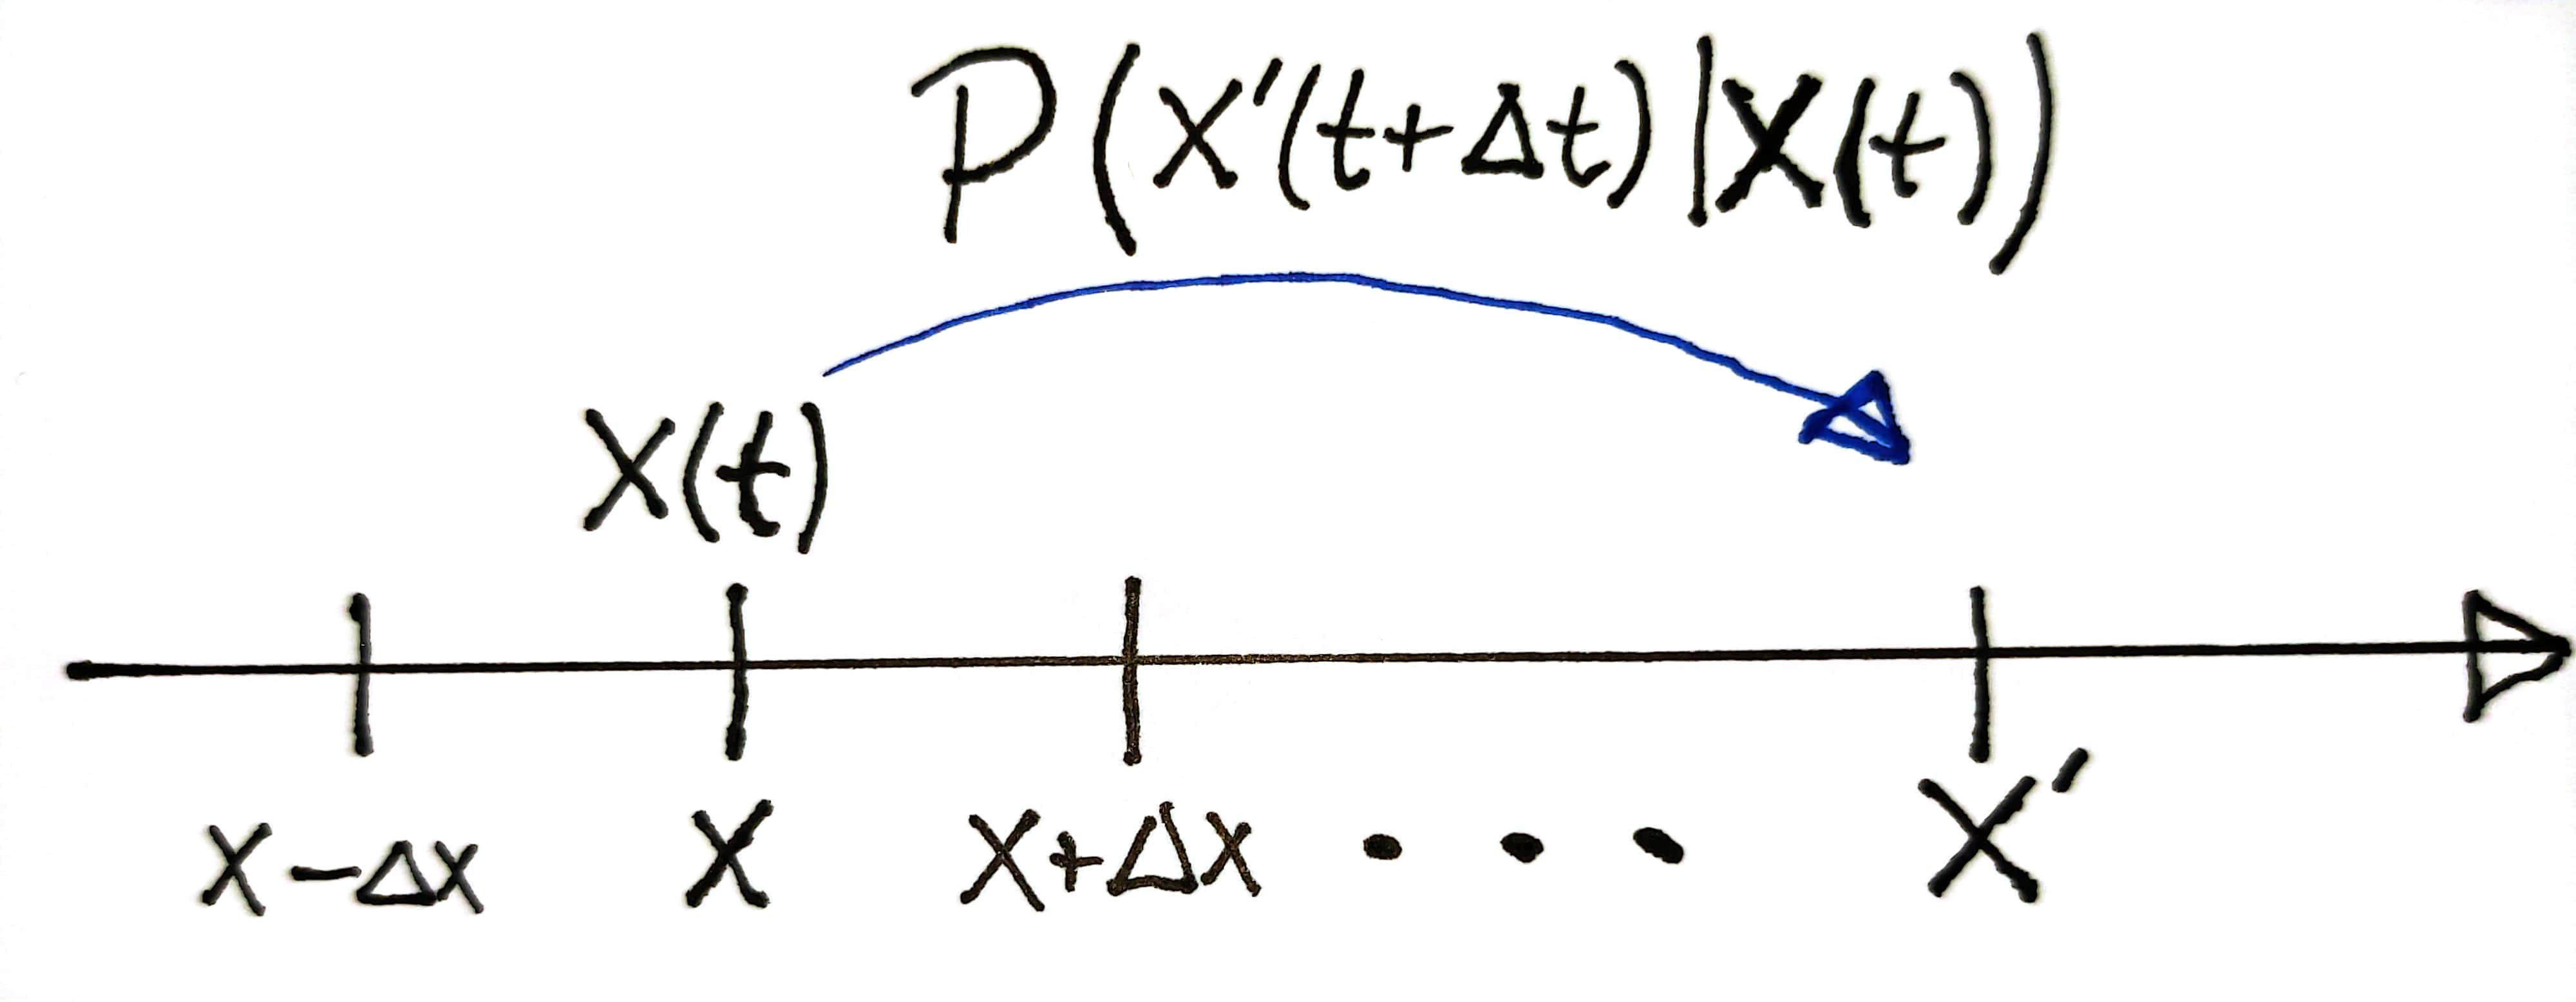
\includegraphics[width=.4\textwidth]{fig/fig1.jpg}
    \caption{Illustration of a stochastic process}
    \label{fig: stochastic process}
\end{figure}


A \emph{Markov process} is a stochastic process with ``no memory''.
This means that, if we have $n$ steps of the process, denoted $x(t_1), x(t_2), \dots x(t_n)$, then the conditional probability of observing $x(t_n)$ given $x(t_1), \dots x(t_{n-1})$, only depends on the last step $x(t_{n-1})$.
This can be stated as
%
\begin{align}
    P(x_n |x_{n-1}, x_{n-2}, \cdots, x_1) = P(x_n | x_{n-1}).
\end{align}
%
Here, we use the shorthand $x_i = x(t_i)$.

As far as we know, the underlying laws of physics are fully described at each time-step, so the question of whether we can model a process as Markovian depends on our description.
For example, if try to describe the flight of a football through the air with only its position, the description is not Markovian, as we need the current velocity to know where it will be at the next time-step.
But, if we include the velocity in our description, the model is Markovian.
A non-Markovian description thus indicate that we have excluded degrees of freedom that contain information about the system.
Be aware that a system being Markovian does not imply statistical independence, so $P(x_{n}, x_{n-1})\neq P(x_n)P(x_{n-1})$


From the definition of conditional probability, \autoref{eq: cond prob}, we can derive that the joint probability of three sequential events, $x_1$, $x_2$ and $x_3$ is given by
%
\begin{align}
    P(x_1, x_2, x_3) = P(x_3|x_2,x_1)P(x_2|x_1)P(x_1).
\end{align}
%
A Markovian process thus has the property
%
\begin{align}
    P(x_1, x_2, x_3) = P(x_3|x_2)P(x_2|x_1)P(x_1).
\end{align}
%
We can furthermore write $P(x_3, x_1) = \sum_{x_2 \in \Ex} P(x_3, x_2, x_1)$.
From this, we derive the Chapman-Kolmogorov equation,
%
\begin{align}\label{eq: chapman kolmogorov}
    P(x_3|x_1) = \sum_{x_2} P(x_3|x_2) P(x_2|x_1).
\end{align}
%
By repeatedly applying this process, we can get conditional probability between two steps $x_1$ and $x_{n+1}$ arbitrarily far removed,
%
\begin{align}\label{eq: cond prob markov x0 given xn}
    P(x_{n+1}|x_1) 
    = \sum_{ x_2, \dots x_n}
    P(x_{n+1}|x_n) P(x_n| x_{n-1})\dots P(x_2|x_1).
\end{align}
%
We see that this already begins to resemble something like a sum over all possible ``paths'' that the proces $x(t)$ can take to transition from $x_1$ at $t_1$ to $x_{n+1}$ at $x(t_{n+1})$.
This is illustrated in \autoref{fig: paths}.


\begin{figure}[!htb]
    \centering
    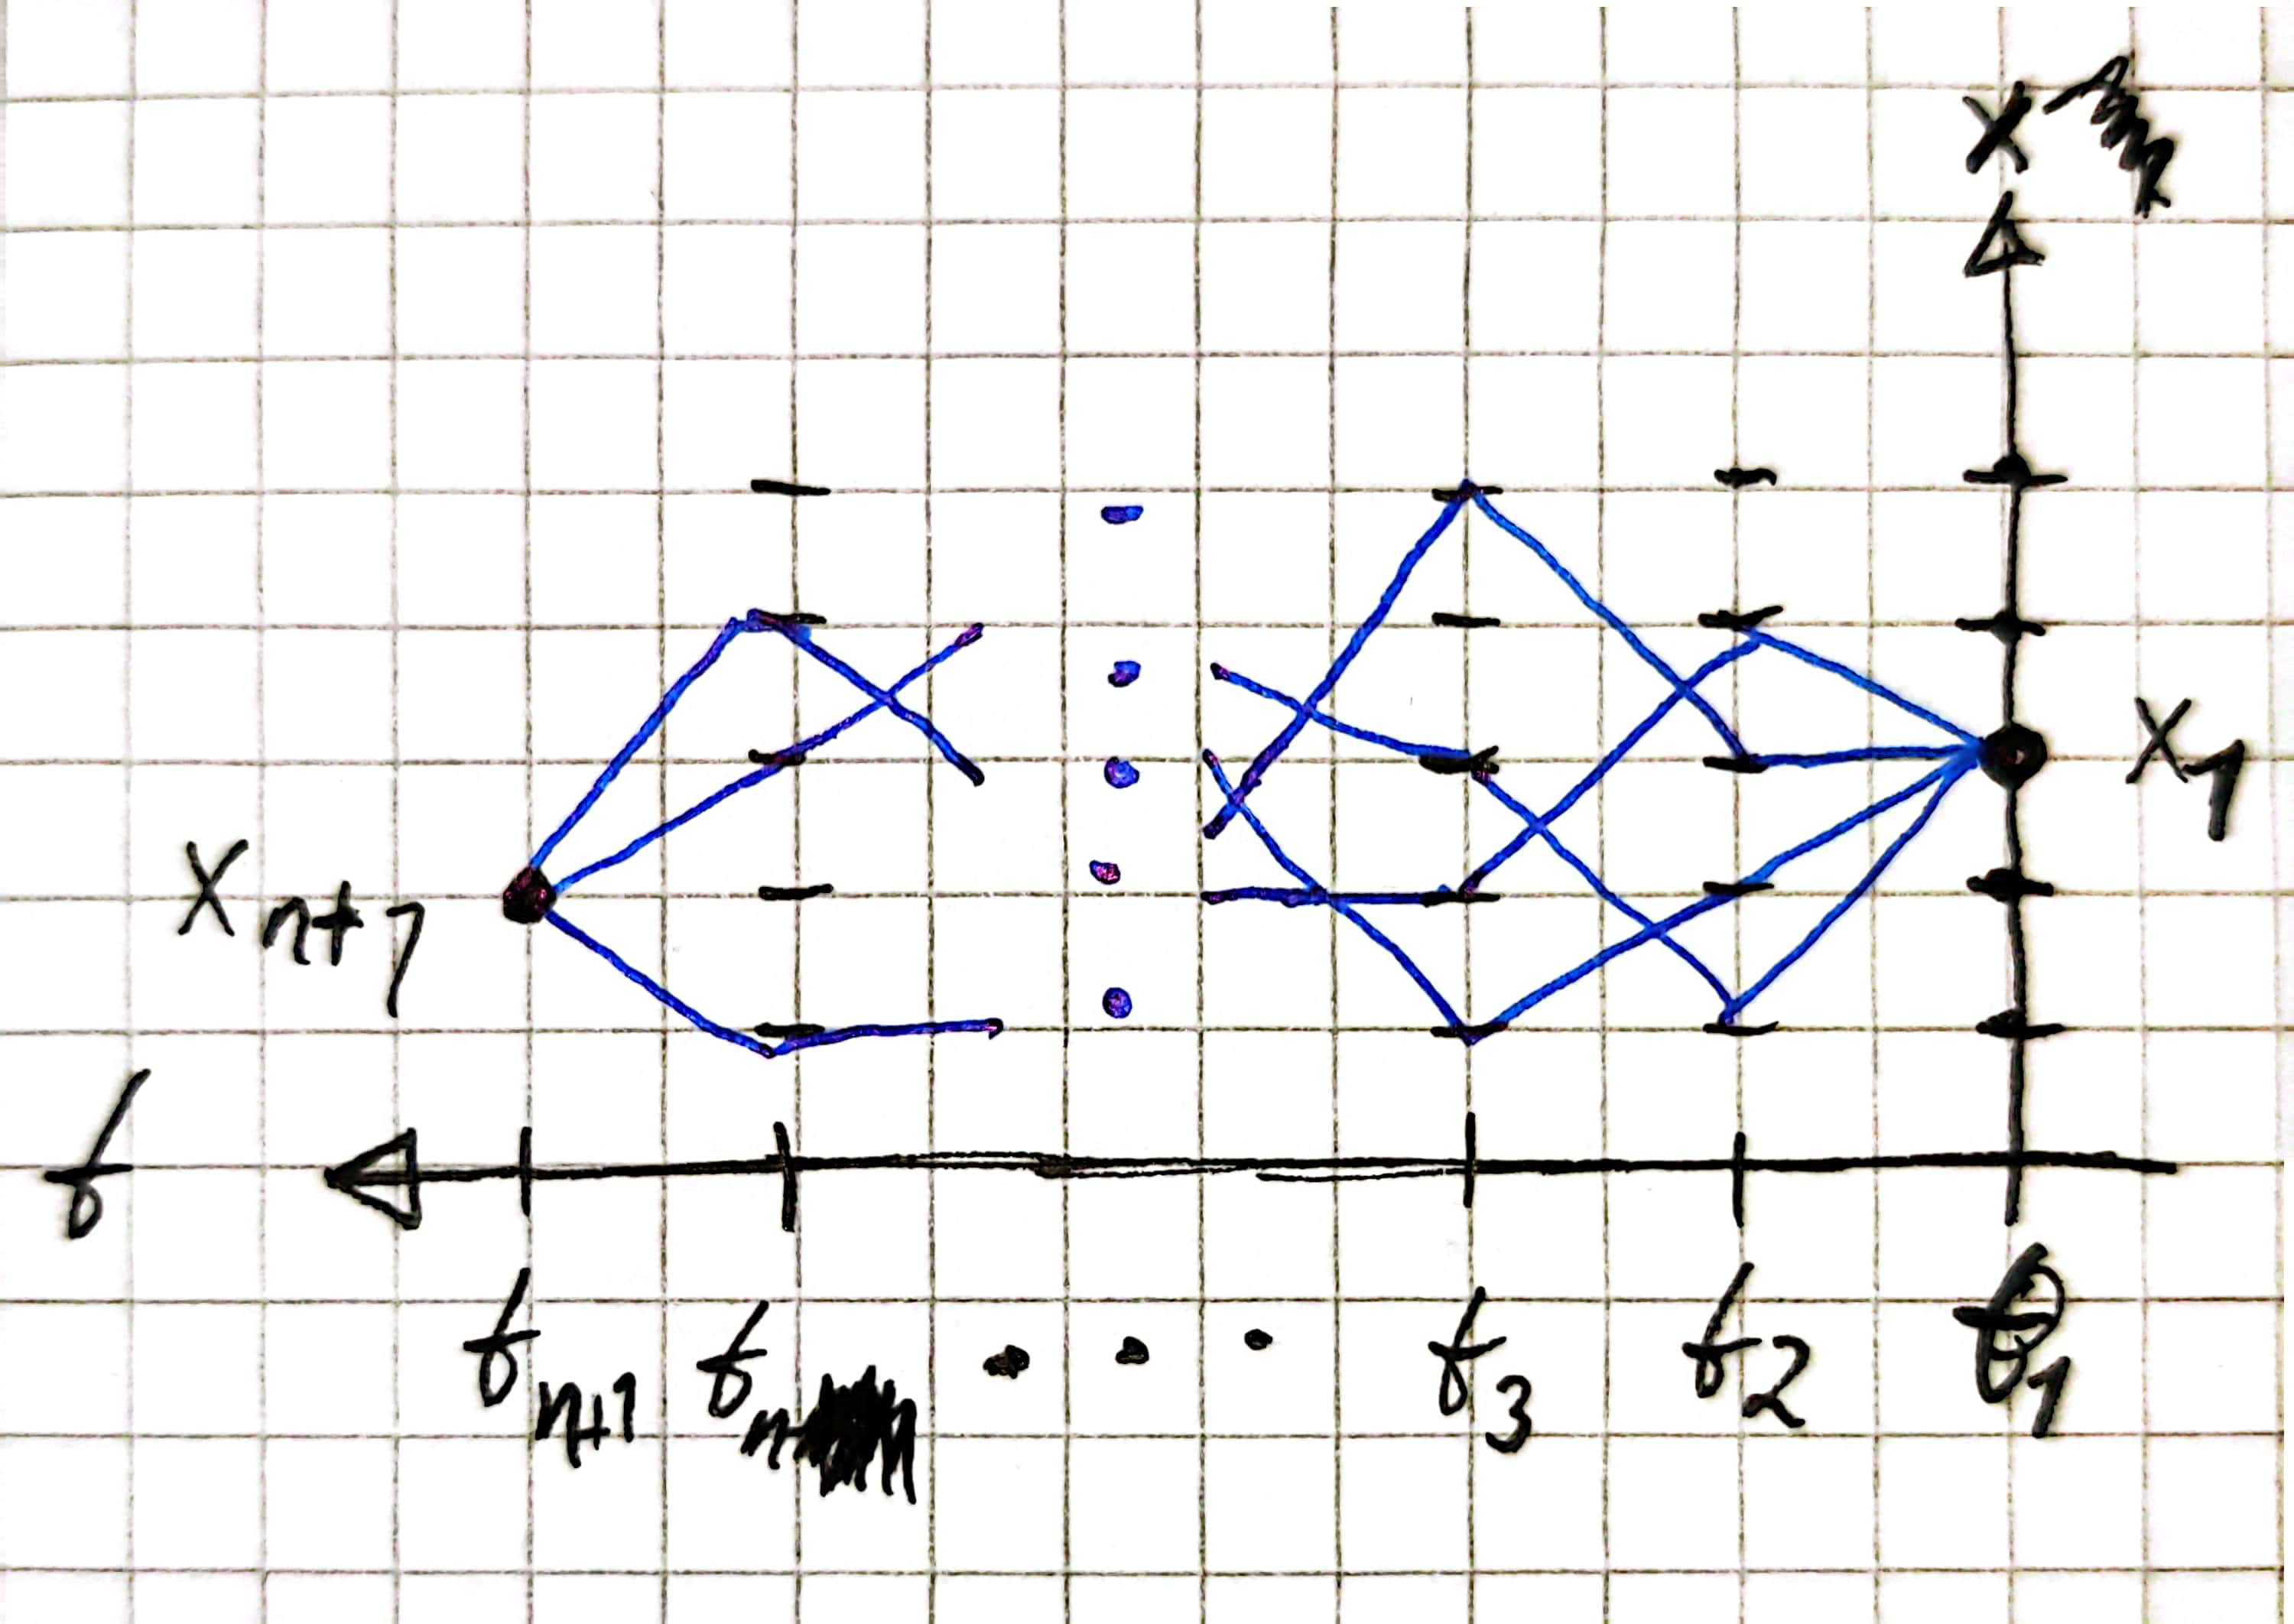
\includegraphics[width=.4\textwidth]{fig/fig2.jpg}
    \caption{Some of the paths between the initial and final state.}
    \label{fig: paths}
\end{figure}


\subsection*{The continuum limit}
\label{subsection: continuum limit}

If we consider a particle on a line instead of a lattice, so $\Ex = \R$, we must consider \emph{probability densities} $\Pe(x)$.
The probability of finding the particle between the points $x_i$ and $x_i + \Delta x$ is, for small $\Delta x$,
%
\begin{align}\label{eq: probability density}
    P(x) \equiv P(x \in [x_i, x_i + \Delta x]) = \Delta x \Pe(x).
\end{align}
%
This corresponds to the limit $\Delta x \rightarrow 0$ for the discrete process considered above, and allows us to go from sums to integrals,
%
\begin{align}
    \sum_{x} P(x) \sim \sum_{x} \Delta x \Pe(x) \underset{\Delta x \rightarrow 0}{\longrightarrow} \int \dd x \, \Pe(x).
\end{align}
%
In this limit the Chapman-Kolgomorov equation, \autoref{eq: chapman kolmogorov}, becomes
%
\begin{align}\label{eq: chapman kolgomorov cont}
    \Pe(x'|x) = \int \dd x'' \, \Pe(x'|x'') \Pe(x''|x),
\end{align}
%
and \autoref{eq: cond prob markov x0 given xn} becomes
%
\begin{align}\label{eq: cond prob markov x0 given xn cont}
    P(x_{n+1}|x_1) 
    = \left(\int \prod_{i=2}^{n} \dd x_i\right)
    \Pe(x_{n+1}|x_n) \Pe(x_n| x_{n-1})\cdots \Pe(x_2|x_1).
\end{align}

Likewise, we can take the limit $\Delta t\rightarrow 0$, corresponding to $n\rightarrow\infty$, to obtain a process with continuous time.
In this case (the ``continuum limit'') \autoref{eq: cond prob markov x0 given xn cont} becomes
%
\begin{align}\label{eq: general path integral}
    P(x(t_0 + T) | x(t_0) ) 
    &
    =
    \lim_{
        \substack{\Delta x \rightarrow 0\\n\rightarrow \infty}
    }
    \left(\int \prod_{i = 1}^{n} \dd x_i C_n\right)
    \Phi_n(\{x_i\})
    \equiv
    \int \D x(t) \, \Phi[x(t)].
\end{align}
%
where $\Delta t = T/n$ and $t_i = t_1 + (i-1)\Delta t$.
We have defined 
%
\begin{align}
    \Phi(\{x_i\}) = \frac{1}{C_n} \Pe(x(t_{n+1}) | x(t_n) ) \cdots \frac{1}{C_n} \Pe(x(t_{2}) | x(t_1) ),
\end{align}
%
where $C_n$ is a constant we will come back to later.
In the last equality, we have defined the \emph{path integral measure} $\D x(t) = \lim_{n \rightarrow \infty} \prod_{i=1}^n \dd x(t_i) C_n$,
and the \emph{functional} $\Phi[x(t)]= \lim_{n \rightarrow \infty} \Phi_n(\{x_i\})$ emerging from the infinite product of conditional probabilities.
This is a functional and not a function, as it itself takes as its argument a function $x(t)$ and returns a number.
We see that \autoref{eq: general path integral} gives the conditional probability for $x(t_0 + T)$ given $x(t_0)$ by integrating over all possible paths $x(t)$ weighted by $\Phi[x(t)]$.
For now, this is a very formal quantity.
To see the power of this formalism, we consider a concrete process, the Ornstein-Uhleneck process.



\section{Gaussian processes and the Ornstein-Uhlenbeck process}
\label{sectoin: gaussian and OUP}

The most important class of stochastic processes, as it is pretty much the only one we can solve, is Gaussian processes, which are processes with probability densities with the form
%
\begin{align}
    \Pe(x_{n+1}|x_n)
    =
    \frac{ 1 }{ \sqrt{ 2 \pi \sigma_{n+1} } }
    \exp \left\{ {-\frac{(x_{n+1} - \bar x_{n + 1})^2}{2 \sigma_{n+1} }} \right\}
\end{align}
%
Here, $\bar x_{n+1}$ is the expected value of $x_{n+1}$, and $\sigma_{n+1}$ the variance.
As we consider Markovian processes, these quantities are functions of (equivalently, conditioned on) only the previous step, $x_n$.


If we have a vector valued process instead, $\bm x(t) = x_a(t) \hat {\bm x}_a$, then the probability distribution is a multivariate Gaussian
%
\begin{align}
    P(x_{n+1}|x_n)
    = 
    \frac{ 1 }{ \sqrt{ 2 \pi \det \Sigma } }
    \exp \left\{ - \frac{1}{2}\sum_{ab} \left[x_a(t_{n+1}) - \bar x_a(t_{n+1})\right] \Sigma_{ab}^{-1} \left[x_b(t_{n+1}) - \bar x_b(t_{n+1})\right] \right\}.
\end{align}
%
Here, $\Sigma$ is the covariance matrix of $x$.
An example of this may be a particle moving in three dimensions, so $\bm x$ is a three-dimensional vector, or a set of $N$ particles with position and velocity in three dimensions, so $\bm x$ is a $6 N$ component vector.


A specific example is the Ornstein-Uhlenbeck (OU) process, which in one dimension is
%
\begin{align}\label{eq: OUP}
    \odv{ x(t) }{ t } = - \mu x(t) + \eta(t).
\end{align}
%
This models, for example, a particle on a spring in a fluid with thermal noise where friction dominates and inertial effects are negligible.
The linear restoring term $-\mu x(t)$ is from Hooks law, and $\eta(t)$ is a zero-mean random force modeling the forces of the fluid particles bumping into the particle.
You can read more about this process in~\footnote{\url{https://iopscience.iop.org/article/10.1088/1367-2630/ad7ef1/meta}}.
For small $\Delta t$, the expectation value of the OU-process at time $t_{n+1}$ conditioned on $x(t_n)=x_n$ is $\bar{x}_{n+1} = x_n - \mu x_n \Delta t$ --- i.e. where it was the step before minus the correction due to the spring-force.
The variance is $\sigma_{n+1} = 2D \Delta t$, where $D$ is the diffusion constant, which is the variance of the noise $\eta$. Note that this latter quantity does not depend on $x_n$.
With this, OU-process has the conditional probability density for small $\Delta t$
%
\begin{align}
    \Pe(x_{n + 1}| x_n) 
    = \sqrt{ \frac{ \mu }{ 4 \pi D \Delta t } }
    \exp \left\{ -
    \frac{ \left(x_{n + 1} - x_n + \mu x_n \Delta t\right)^2 }{ 4 D \Delta t } 
    \right\}
    = \sqrt{ \frac{ \mu }{ 4 \pi D \Delta t } }
    \exp \left\{ 
    - \frac{ \Delta t }{ 4 D }  \left(\dot x_{n + 1} + \mu x_n\right)^2
    \right\},
\end{align}
%
where we have introduced the discrete time-derivative, $\dot x_{n+1} = (x_{n + 1} - x_n) / \Delta t$.
In the $\Delta t \rightarrow 0$ limit, this becomes a regular derivative.



Inserting the OU process into \autoref{eq: cond prob markov x0 given xn} and taking the continuum limit as discussed above, we get
%
\begin{align}\label{eq:om_func}
    P(x_{n+1}|x_{1})
    & =
    \sum_{x_2\cdots x_{n}}
    \Delta x \Pe \left( x_{n+1}| x_{n} \right) \cdots \Delta x \Pe \left( x_{2}| x_{1} \right)\\
    &
    = \sum_{x_2\cdots x_{n}} \left( \frac{\Delta x}{C_n} \right)^n \exp \left\{ - \frac{\Delta t}{4 D} \sum_n \left[\dot x_{n + 1} - \mu x_n \right]^2 \right\}\\
    & 
    \underset{\substack{\Delta x \rightarrow 0\\ n \rightarrow \infty} }{ \sim }
    \int \D x(t) \,
    \exp \left\{ 
        - \frac{ 1 }{ 4D } 
        \int\limits_{t_1}^{t_{n+1}} \dd t \left[\dot x(t) - \mu x(t)\right]^2
        \right\}
    \equiv
    \int \D x(t) \, \Phi[x(t)].
\end{align}
%
In this case, the integration measure is
%
\begin{align}
    \D x(t) \equiv \lim_{\substack{\Delta x \rightarrow 0\\ n \rightarrow \infty} } \prod_{n} \Delta x \sqrt{ \frac{\mu}{ 4 \pi D \Delta t }},
\end{align}
%
which corresponds to $C_n = \sqrt{\mu/4\pi D \Delta t}$.
This measure is not strictly well-defined. 
To performed calculations, we will have re-descritize the path integral, so this can be considered as a notational trick rather than a true limit. The functional $\Phi[x(t)]$ in Eq.~\eqref{eq:om_func} is often referred to as the Onsager-Machlup functional, thanks to its appearance in a 1953 paper by the two physicists. We'll come back to it later on in the course.


\section{Master equation}
\label{section: master equation}

We will here consider stochastic processes using a different formalism, the master equation. While this formalism will be relevant later on in the course, we introduce it early on to make a point about the equivalence between the path integral representation of stochastic process and other, more common approaches.
If we consider a discrete stochastic process $N(t)$, and Taylor-expand the conditional probability of $N'$ at $t + \Delta t$ given $N$ at $t$ in small $\Delta t$, we get
%
\begin{align}\label{eq: expansion cond prob}
    P(N'(t + \Delta t)| N(t)) = 
    \underbrace{P(N'(t)|N(t))}_{\delta_{N'N}} + \Delta t 
    \underbrace{\pdv{P(N'(t')|N(t))}{t'}\bigg|_{t'=t}}_{W_t(N'|N)} + \Oh(\Delta t ^ 2).
\end{align}
%
Here, we define the \emph{transition rates} $W_t(N'|N)$. The subscript highlights the fact that these may explicitly depend on time: for example, if the stochastic process $N(t)$ describes the number of individuals in the population of a particular species of insects, the transition rates $W_t(N+1|N)$ and $W_t(N-1|N)$ associated with birth and death processes might depend explicitly on time through seasonal variations in temperature.

The transition rate $W_t(N'|N)$ can be considered as a matrix, 
%
\begin{align}
    W_t(N'|N) = 
    \begin{pmatrix}
        W_t(1|1) & W_t(1|2)& W_t(1|3) &\cdots\\
        W_t(2|1) & W_t(2|2)& W_t(2|3) &\cdots \\
        W_t(3|1) & W_t(3|2)& W_t(3|3) &\cdots \\
        \vdots & \vdots & \vdots & \ddots
    \end{pmatrix},
\end{align}
%
where the entries are the rate at which state $N$ transitions to state $N'$.
If we consider $N' = N$, then we can, by the principle of total probability (the probability of all possible outcomes add up to one), write
%
\begin{align}
    P(N(t + \Delta t)| N(t)) = 1 + \Delta t W_t(N|N) 
    = 1 - \sum_{N' \neq N}P(N'(t + \Delta t)| N(t))
    = 1 - \sum_{N' \neq N}\Delta t W_t(N',N),
\end{align}
%
or equivalently
%
\begin{align}\label{eq: rate cons condition}
    W_t(N|N) = - \sum_{N'\neq N}W_t(N'|N).
\end{align}
%
This insures the conservation of probability.
If we consider the matrix form of the rates, this means the diagonals of $W_t(N'|N)$ are given by minus the sum of the off-diagonal elements in each column,
%
\begin{align}
    W_t(N'|N) = 
    \begin{pmatrix}
        - \sum_{N\neq 1} W_t(N|1) & W_t(1|2)& W_t(1|3) &\cdots\\
        W_t(2|1) & - \sum_{N\neq 2} W_t(N|2)& W_t(2|3) &\cdots \\
        W_t(3|1) & W_t(3|2)& - \sum_{N\neq 3} W_t(N|3) &\cdots \\
        \vdots & \vdots & \vdots& \ddots 
    \end{pmatrix},
\end{align}
%
If we expand the Chapman-Kolmogorov, \autoref{eq: chapman kolmogorov},
%
\begin{align}
    P(N(t_3) |N(t_1))
    & =
    \sum_{N(t_2)} 
    \left[
        \delta_{N(t_3)N(t_2)}
        + (t_3 - t_2) W_{t_2}(N(t_3)|N(t_2))
    \right]
    P(N(t_2)|N(t_1))
    \\
    & =
    (t_3 - t_2)\sum_{N(t_2)\neq N(t_3)} 
        W_{t_2}(N(t_3)|N(t_2)) P(N(t_2)|N(t_1))\\
    & \quad 
    + \left[ 1 + (t_3 - t_2) W_{t_2}(N(t_3)|N(t_2)=N(t_3))  \right] P(N(t_2)=N(t_3)|N(t_1))
\end{align}
%
If we apply \autoref{eq: rate cons condition}, and define $\Delta t = t_3 - t_2$, we can rearrange this to read
%
\begin{align}
    &\frac{P\left(N(t_3)|N(t_1)\right) - P(N(t_2)=N(t_3)|N(t_1))}{\Delta t}\\
    &=
    \sum_{N(t_2) \neq N(t_3)}
    \left[
        W_{t_2}(N(t_3)|N(t_2))P(N(t_2)|N(t_1))
        - W_{t_2}(N(t_2)|N(t_2)=N(t_3))P(N(t_2)=N(t_3)|N(t_1))
    \right]
\end{align}
%
The top line of this equation is the difference in probability of finding the system in the state $N(t_3)$ at time $t_3$ and $N(t_2)$, so in the limit $\Delta t \rightarrow 0$ becomes a derivative.
On the bottom, we have the difference between the \emph{gain} rate and the \emph{loss} rate in to and out of state $N(t_3)$
We take the limit, which gives the \emph{master equation},
%
\begin{align}
    \odv{}{t} P(N(t)|N_0) =
    \sum_{N'\neq N} \left[
        W_t(N(t)|N'(t))P(N'(t)|N_0)
        - 
        W_t(N'(t)|N(t))P(N(t)|N_0)
    \right].
\end{align}
%
Solving for $P(N(t)|N_0)$ by integrating the master equation will of course give the same result as computing the conditional probability by means of the corresponding path integral, since both are directly derived from the definition of the conditional probability distribution only by assuming the process is Markovian.
Although the two formulations are equivalent, they may be better or worse suited for different problems.

\begin{framed}
    \noindent
    \textbf{The quantum-stochastic analogy}\\
    The master equation is a first-order linear ODE giving the time-evolution of a probability distribution.
    If this reminds you of the Schrödinger equation for the quantum mechanical wave function, the similarities does not stop here.
    In fact, the correspondence between the master equation and the Onsager-Machlup functional is analogous to the relationship between the Schrödinger and the Feynman path integral in QM. Let's briefly revisit the latter.
    The classical action of a process is a functional
    %
    \begin{align}
        S[x] = \int\limits_{t_a}^{t_b} \dd t \, L(x, \dot x, t), 
    \end{align}
    %
    where $L = V - T$ is the Lagrangian.
    In classical mechanics, the motion is determined by the Euler-Lagrange equations, $\fdv{ S }{ x(t) } = 0$, while in quantum-mechaics, the amplitude for a process is, according to the Feynman path integral,
    %
    \begin{align}
        K(x_b | x_a) &= \sum_{\mathrm{paths}\, x} \Phi[x], & \Phi[x] \propto e^{iS[x] / \hbar}~.
    \end{align}
    %
    The Schrödinger equation gives the equivalent evolution of the wave-function,
    %
    \begin{align}
        i \hbar \odv{  }{ t } \Psi(x(t)) = \hat H \Psi(x(t)),
    \end{align}
    %
    where $\hat H$ is the Hamiltonian operator, and the amplitude is the overlap between the initial and finite wave-functions, $K(x_b | x_a) = \braket{ \Psi(x(t_b)) | \Psi(x(t_a)) } $. Just like the master equation can be derived from the Chapman-Kolmogorov equation, so can the Schrödinger equation be derived from the Feynman path integral representation of the process by expanding the latter in small $\Delta t = t_b - t_a$. If you want to read more about the Feynman path integral, this is discuss very nicely in the related textbook by Feynman and Hibbs (available for free online).
\end{framed}




\section{Gaussian (path) integrals}

The most important integrals we will meet are \emph{Gaussian integrals}.
The simplest Gaussian integral, which will be the basis for this section, is
%
\begin{align}\label{eq: gaussian integral}
    \int\limits_{-\infty}^\infty \dd x \, e^{-\frac{1}{2} a x^2} = \sqrt{ \frac{ 2 \pi  }{ a }}.
\end{align}
%
The reason we can solve Gaussian processes, as we mentioned earlier, is that we can solve Gaussian integrals.
With this simple result, we can solve path integrals over spaces of functions.
Consider the following object, 
%
\begin{align}
    Z = \int \D \phi
    \exp \left\{ 
        - \frac{1}{2} \int \dd t_1 \dd t_2 \, 
        \sum_{ab}
        \phi_a(t_1) \tilde{A}_{ab}(t_1, t_2) \phi_b(t_2)
    \right\}.
\end{align}
%
Here, $\phi(t_1)$ is a vector function with $d$ components, $\phi_a(t) = (\phi_1(t), \phi_2(t)\dots)^T$, and $\tilde{A}_{ab}(t_1, t_2)$ is a matrix-function, which we assume to be symmetric with respect to both component and time indices.
This can be done without loss of generality, as any antisymmetric part of $A$ does not contribute to the quadratic form $\phi^T A \phi$.
%In the case of Markov-processes, $A(t_1, t_2)$ will be \emph{time-local}, meaning $A(t_1, t_2) = A(t_1) \delta(t_1 - t_2)$.
For the path integral $Z$ to be well-defined, we must discretize $t_n = n \Delta t$, with $n \in \Z$
This gives us an extra set of indices, $\phi_a(t_i) = \phi_{a,i}$.
However, we can deal with this by ``unpacking'' the two-dimensional structure of $\phi_{a,i}$,
%
\begin{align}
    \phi_\alpha = 
    \left[\phi_1, ... \phi_N\right]
    =
    \left[
        \phi_{1, 1}, \phi_{2, 1}\dots\phi_{d,1}, \phi_{1, 2}\dots\phi_{d, n}
    \right],
\end{align}
%
where $N = d \times n$.
This is analogous to ``flattening'' an array in computer programming.
We also apply this to $\tilde{A}_{ab}(t_1,t_2) \to \tilde{A}_{\alpha\beta}$.
Absorbing the factor $\Delta t^2$ coming from the integration into a redefinition of $\tilde{A} = A/\Delta t^2$,
% The discretized Dirac-delta is $\delta(t_1 - t_2) \sim \frac{1}{\Delta t} \delta_{t_1, t_2}$, so factoring out this $\Delta t$ we get 
% %
% \begin{align}
%     A_{ab}(t_1,t_2)
%     \sim \frac{1}{\Delta t} A_{ab,ij}
%     \rightarrow \frac{1}{\Delta t} A_{\alpha \beta},
% \end{align}
%
the path-internal then discretizes as 
%
\begin{align}
    Z_0 = \int \left( \prod_{\alpha=1}^N \dd \phi_\alpha \right) \, 
    \exp \left\{ 
        - \frac{1}{2} \sum_{\alpha \beta} 
        \phi_\alpha A_{\alpha \beta} \phi_\beta
    \right\}.
\end{align}
%
We now assume $A$ is diagonalizable, so we can write it as $A = G \Lambda G^{-1} $, where $\Lambda = \mathrm{\lambda_1, ... \lambda_N}$ is diagonal, with $\lambda_\alpha$ are the eigenvalues of $A$. Based on our earlier assumption of symmetry we have that $G^{-1}=G^T$ is a rotation, hence ${\rm det}(G)=\pm 1$.
We can therefore perform a change of variables, $z = G^{-1}\phi$, which comes with a Jacobian of unity and simplifies the integral
%
\begin{align}\label{eq: gaussian integral}
    Z_0 
    = 
    \int \left( \prod_{\alpha=1}^N \dd z_\alpha \right)
    \exp \left\{ - \frac{1}{2} \sum_{\alpha} \lambda_\alpha z_\alpha^2 \right\}
    =
    \sqrt{ \det 2 \pi A^{-1} }.
\end{align}
%
Here, we factored the exponential, used the simple Gaussian integral \autoref{eq: gaussian integral}, and used the fact that the product of the eigenvalues is the determinant. 

%%%%%%%%%%%%%
% Lecture 2 %
%%%%%%%%%%%%%

The next generalization we do, is to introduce a ``source'' $J$, which gives the \emph{moment generating function}
%
\begin{align}\label{eq: generating functional}
    Z[J] = \int \left(\prod_\alpha  \dd \phi_\alpha \right) \exp \left\{ - \frac{1}{2} \sum_{\alpha \beta} \phi_\alpha A_{\alpha \beta} \phi_\beta + \sum_\alpha J_\alpha \phi_\alpha \right\}.
\end{align}
%
For $J = 0$, this reduces to the integral above.
However, we can evaluate this integral explicitly, which yields
%
\begin{align}
    Z[J] = Z_0 \exp \left\{ \frac{ 1 }{ 2 }  \sum_{\alpha \beta} J_\alpha A_{\alpha \beta}^{-1} J_\beta \right\}.
\end{align}
%

\begin{framed}\noindent
\textit{Exercise}: Evaluate the integral in \autoref{eq: generating functional}.
If you \emph{complete the square} by introducing a shifted integration variable $\phi'$, so that the argument of the exponential takes the form $\phi' A \phi' + \const$, you can again use Gaussian integral formula \autoref{eq: gaussian integral}.
\end{framed}

With this result, we can compute arbitrary expectation values of products of fields.
If the probability density of $\phi_\alpha$ is given by
%
\begin{align}
    \Pe(\phi) = \frac{1}{Z_0} \exp \left\{ \frac{1}{2} \sum_{\alpha \beta} \phi_{\alpha} A_{\alpha \beta} \phi_\beta \right\},
\end{align}
%
then
%
\begin{align}
    \E{ \phi_{K_1} \phi_{K_2} \cdots \phi_{K_{2n}} }
    & = 
    \int \left( \prod_{\alpha=1}^N \dd z_\alpha \right)\, 
    \phi_{K_1} \phi_{K_2} \cdots \phi_{K_{2n}}
    \exp \left\{ - \frac{1}{2} \sum_{\alpha} \lambda_\alpha z_\alpha^2 \right\}\\
    & =
    \left[\frac{1}{Z[0]} \pdv{ }{ J_{K_1} } \pdv{ }{ J_{K_2} } \cdots \pdv{ }{ J_{K_{2n}} }Z[J]\right]_{J = 0},
\end{align}
%

As an example, we compute the ``two-point function'' by Taylor-expanding the exponential in the generating functional:
%
\begin{align}
    \E{\phi_{K_1} \phi_{K_2}} 
    &
    = 
    \left[
        \pdv{ }{ J_{K_1} }\pdv{ }{ J_{K_2} }
        \left\{
            1
            + \frac{1}{2}\sum_{\alpha \beta} J_\alpha A_{\alpha \beta}^{-1} J_\beta
            + \frac{ 1 }{ 2 } \left(\frac{1}{2}\sum_{\alpha \beta} J_\alpha A_{\alpha \beta}^{-1} J_\beta\right)^2
            + \Oh(J^4)
        \right\}
    \right]_{J = 0} \\
    & = \frac{1}{2}\left(  A_{K_1 K_2}^{-1} +  A_{K_2 K_1}^{-1} \right)
    = A_{K_1K_2}^{-1},
\end{align}
%
where we exploited the assumed symmetry of $A$ for the last equality.
As we set $J = 0$, only term with exactly 2 $J$-factors survive.
In general, for only the terms with equal numbers of ``sources'' $J$ as fields $\phi$ in the expectation value survive.
This is why all expectations with an odd number of fields vanish.
The term $A_{K_1K_2}^{-1}$ has many names, but is often called the ``free propagator''.

If we take a step to four-point functions, things quickly become more complicated.
Explicitly,
%
\begin{align}
    \E{\phi_{K_1} \phi_{K_2} \phi_{K_3} \phi_{K_4}} 
    &
    = 
    \left[
        \pdv{ }{ J_{K_1} }\pdv{ }{ J_{K_2} }\pdv{ }{ J_{K_3} }\pdv{ }{ J_{K_4} }
        \left\{
            \cdots
            + \frac{ 1 }{ 2 } \left(\frac{1}{2}\sum_{\alpha \beta} J_\alpha A_{\alpha \beta}^{-1} J_\beta\right)^2
            \cdots
        \right\}
    \right]_{J = 0} \\
    & = \frac{1}{8}
    \underbrace{
        \left(  A_{K_1 K_2}^{-1} A_{K_3 K_4}^{-1} +  A_{K_1 K_3}^{-1} A_{K_2 K_4}^{-1}  + \cdots\right)
    }_{4! \, \mathrm{terms}}.
\end{align}
%
The terms all have the form $A_{K_i K_j}^{-1} A_{K_k K_\ell}^{-1}$, where $(i,j,k,\ell)$ is some permutation of $(1,2,3,4)$.
There are $4!$ permutations of $4$ terms, which gives the number of terms.
Luckily, there is a lot of redundancy.
For example,
%
\begin{align}
    A_{K_1 K_2}^{-1} A_{K_3 K_4}^{-1} 
    = A_{K_3 K_4}^{-1} A_{K_1 K_2}^{-1} 
    = A_{K_2 K_1}^{-1} A_{K_3 K_4}^{-1} 
    = \cdots.
\end{align}
%
We will introduce the graphical formalism of \emph{Feynman diagrams} to enumerate the distinct terms.

In general, $2n$-point function is
%
\begin{align}\label{eq: Wicks theorem}
    \E{\varphi_{K_1 } \cdots \varphi_{K_{2n}} }
    = 
    \frac{1}{2^n n!} \sum_{\sigma \in S_{2n}}
    A^{-1}_{K_{\sigma(1)} K_{\sigma(2)}} \cdots A^{-1}_{K_{\sigma(2n-1)} K_{\sigma(2n)}}.
\end{align}
%
Here, $\sigma$ is one permutation of the numbers $(1, 2, \dots 2n)$.
It is a bijection of the form
%
\begin{align}
    \sigma : (1, 2, \dots 2n) \longrightarrow (\sigma(1), \sigma(2), \dots \sigma(2n)),
\end{align}
%
which means $i \neq j \Leftrightarrow \sigma(i) \neq \sigma(j)$.
$S_n$ is the set of all such permutations.
The size of this set is $|S_{2n}| = 2n!$.
This set, together with the operation of composition, makes up the discreet \emph{symmetric group} of degree $2n$.
This form result is called \emph{the Wick-Isserlis theorem}, or more commonly \emph{Wick's theorem}.
Wick's theorem serves as the basis for perturbative field theory.
By rewriting non-Gaussian field integrals as infinite sums of Gaussian integral, we are able to systematically approximate much more complicated theories.

As a final note, if we have a generic function $f(\phi)$ of the stochastic variables, we can evaluate expectation values as
%
\begin{align}\label{eq: expectation of f}
    \E{f(\phi)} 
    = \exp 
    \left\{ 
        \frac{ 1 }{ 2 } \sum_{\alpha \beta} A^{-1}_{\alpha \beta} \pdv{  }{ \phi_\alpha } \pdv{  }{ \phi_\beta } 
    \right\} f(\phi) \bigg|_{\phi = 0}.
\end{align}
%
Here, a function of a differential operator is understood to be defined in terms of its Taylor expansion.
\begin{framed}\noindent
    \textit{Exercise:} 
    Derive the form \autoref{eq: expectation of f} using Wick's theorem \autoref{eq: Wicks theorem}.
    Begin by expanding $f$ in a Taylor series.
\end{framed}


\section{Feynman diagrams}

To more efficiently compute expectation value, we represent the propagators $A^{-1}$ as lines connecting points, representing the stochastic variables $\phi_\alpha$.
If we have several variables in an $n$-point function with the same index $K_i$, then this represents the same point, and the line representing the propagator can create a ``loop'' by starting and ending at that point, 
Alternatively, we can create a chain of propagators that starts and end at that point.
As an illustration, we write out the expectation of six fields, where four have the same index:
%
\begin{align}
    \E{\phi_1 \phi_2^4 \phi_3} 
    &=&&
    \parbox{.3\textwidth}{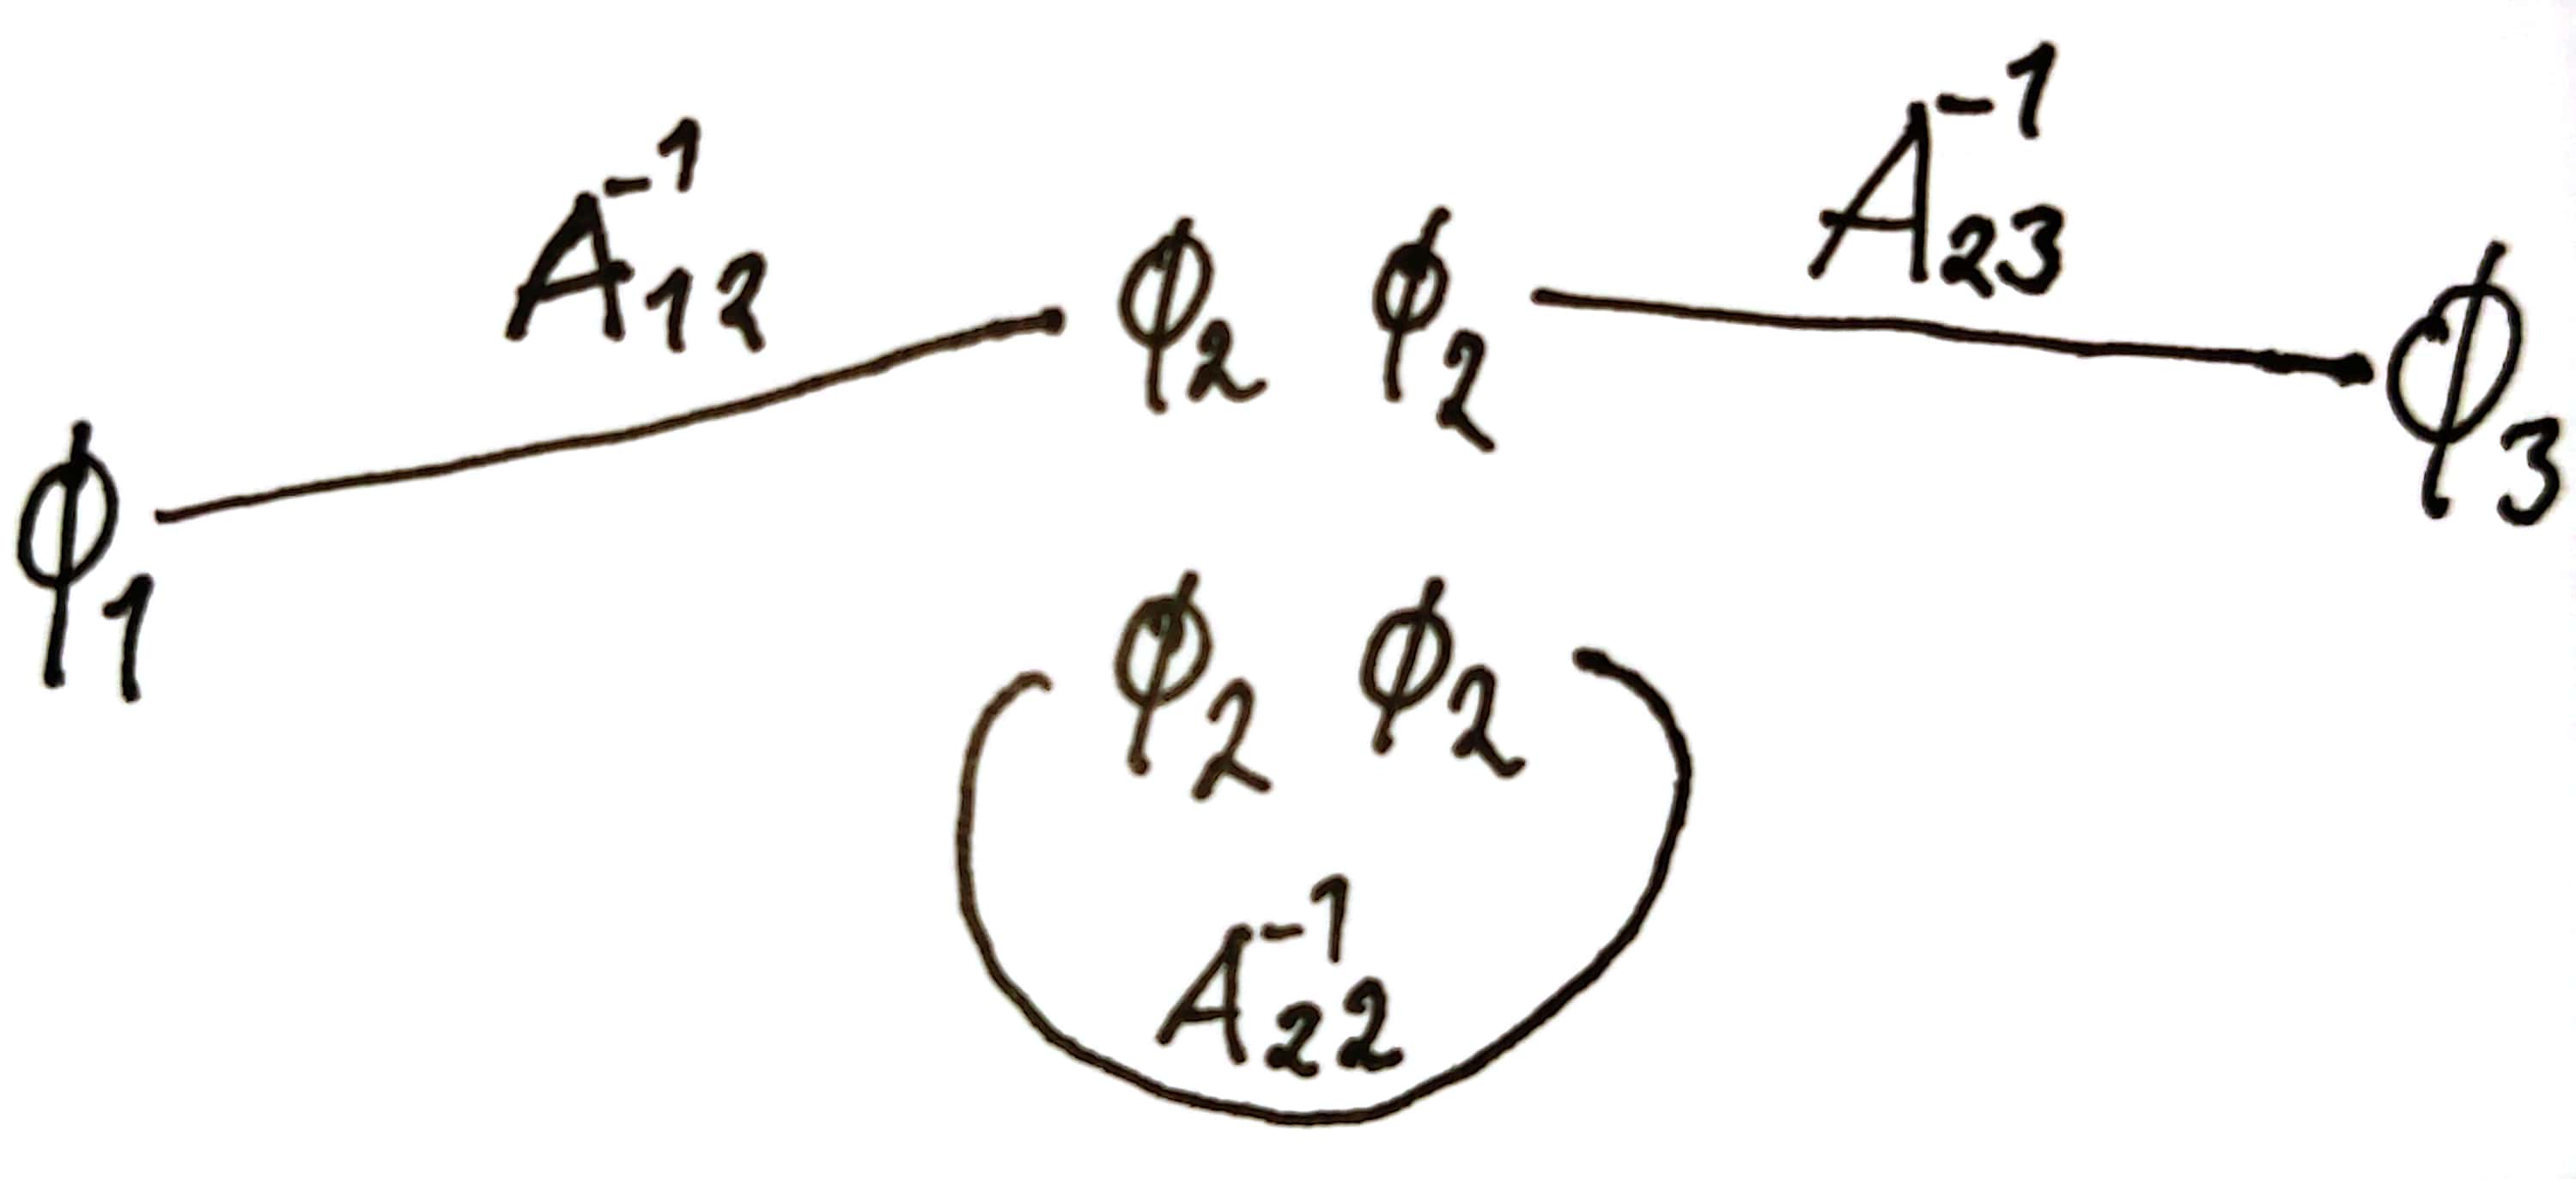
\includegraphics[width=.3\textwidth]{fig/pathint_01.jpg} }
    &&+&&
    \parbox{.3\textwidth}{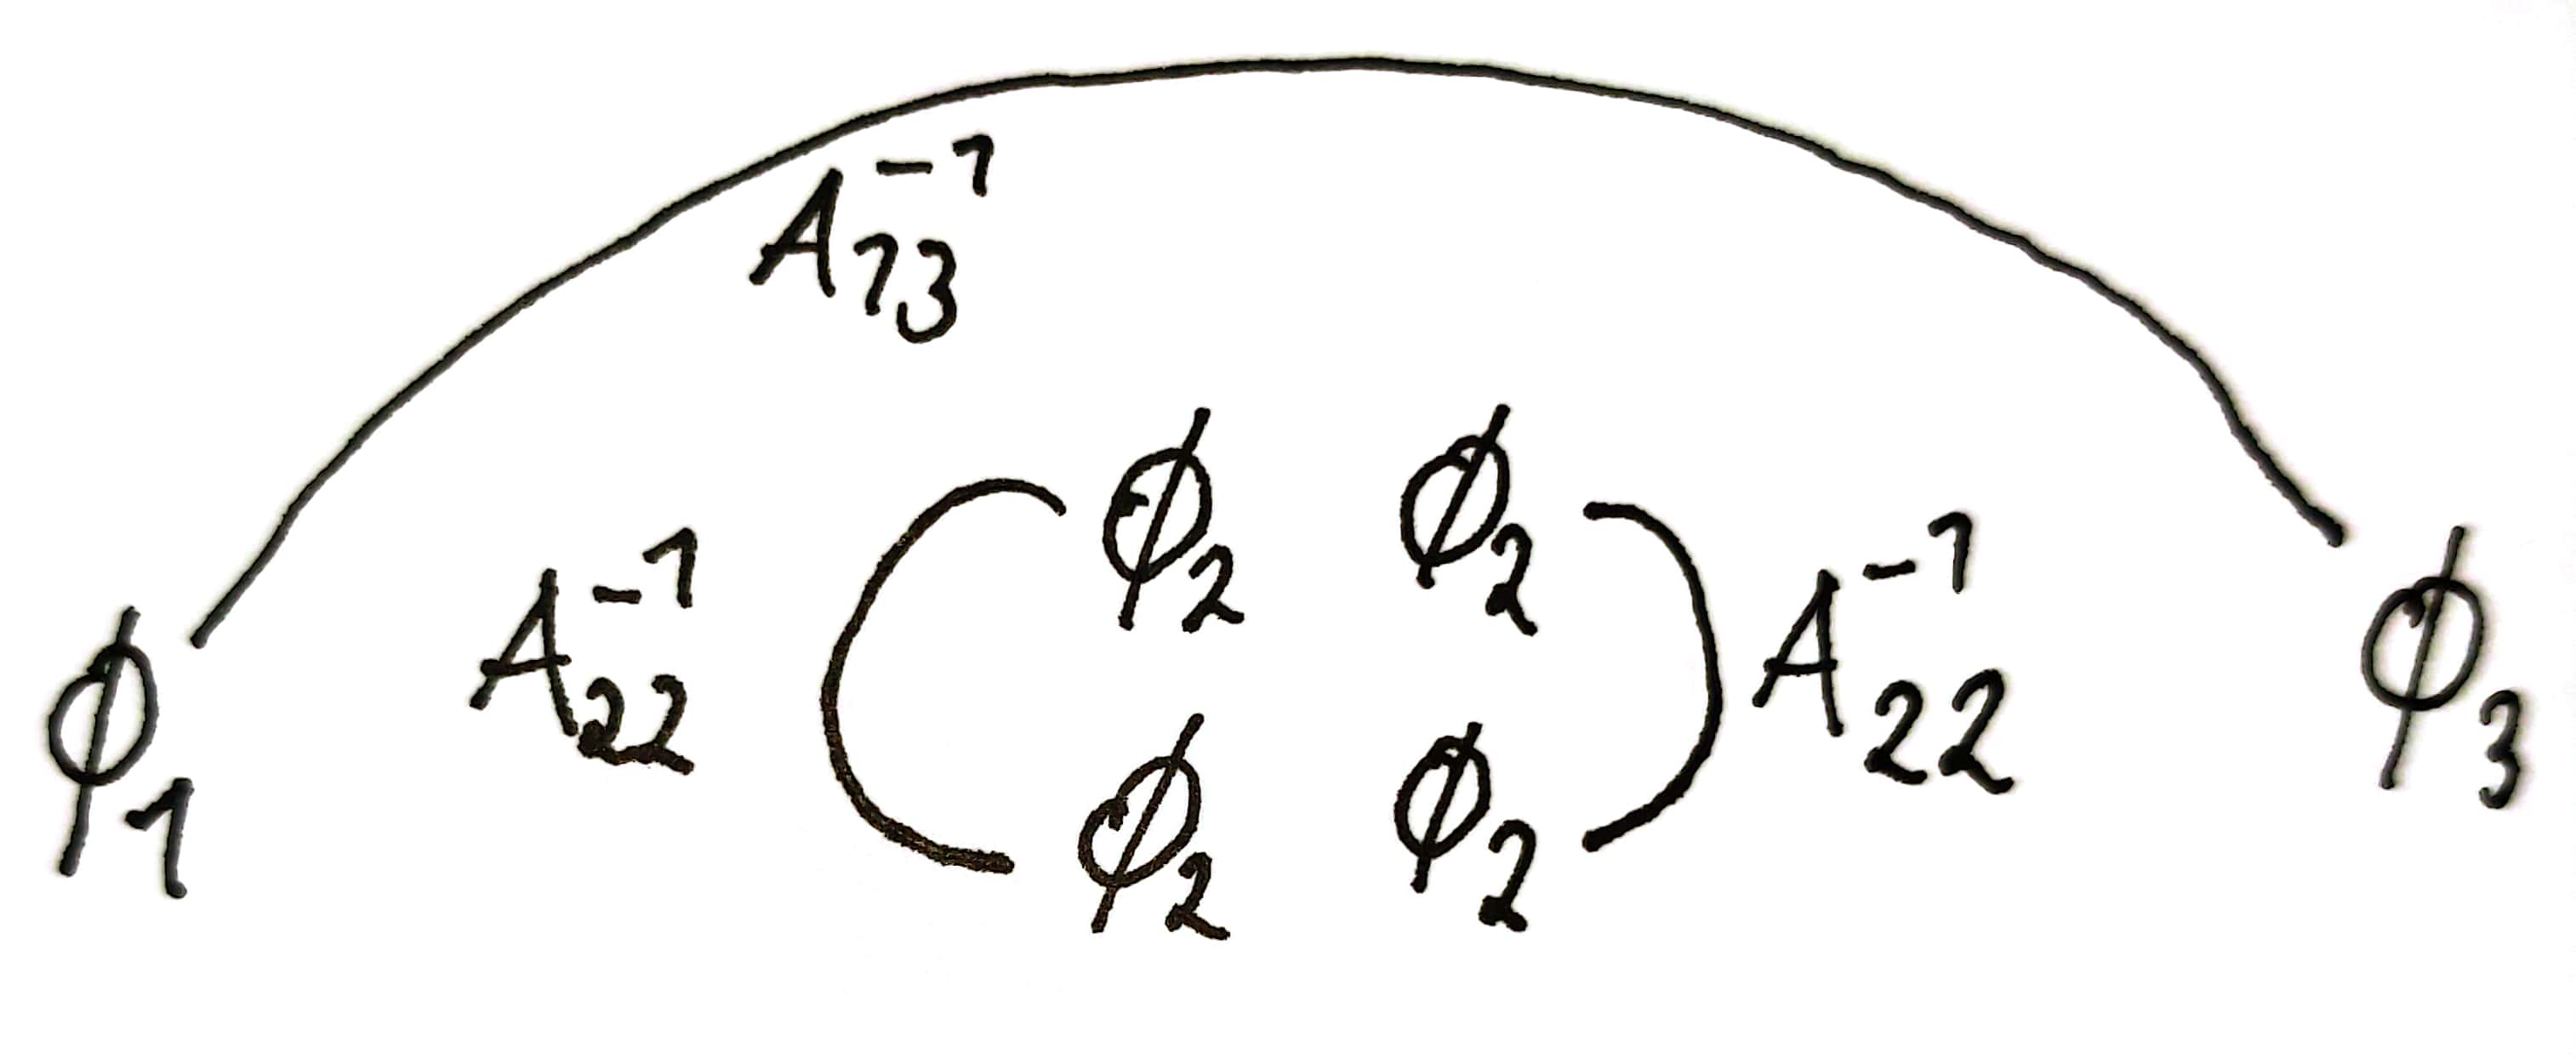
\includegraphics[width=.3\textwidth]{fig/pathint_02.jpg} }\\
    &= &&
    s_1 A_{12}^{-1} A_{22}^{-1} A_{23}^{-1}
    &&+&&s_2 A_{13}^{-1} \left( A_{22}^{-1} \right)^2.
\end{align}
%
Here, $s_1$ and $s_2$ are \emph{symmetry factors}, which count the number of distinct ways we could have created the same diagrams by connecting propagators.
For the first diagram, $\phi_1$ can be connected 4 ways into the cluster, the cluster can self-connect in three different ways, and we are then left with only one way to connect the cluster to $\phi_3$, so $s_1 = 4 \times 3 \times 1 = 12$.
For the second diagram, there is only one way to connect $\phi_1$ and $\phi_3$, then the first connection in the cluster can be done in $3$ ways, and the second is then forced.
This gives $s_2 = 3$.

Feynman diagrams often appear in a more abstract form, where the fields and propagators are implied.
The diagrams illustrated above are then
%
\begin{align}
    \E{\phi_1 \phi_2^4 \phi_3} = 
    \parbox{16mm}{
    \centering
    \begin{fmfgraph*}(16,10)
        \setval
        \fmfleft{i}
        \fmfright{o}
        \fmftop{t}
        \fmf{plain}{i,c,o}
        \fmffreeze
        \fmf{plain,left}{c,t}
        \fmf{plain,left}{t,c}
    \end{fmfgraph*}
    }
    +
    \parbox{16mm}{
    \centering
    \begin{fmfgraph*}(10,4)
        \setval
        \fmfleft{i}
        \fmfright{o}
        \fmf{plain,left}{i,c,o,c,i}
    \end{fmfgraph*}\\
    \begin{fmfgraph*}(16,2)
        \setval
        \fmfleft{i}
        \fmfright{o}
        \fmf{plain}{i,c,o}
    \end{fmfgraph*}
    }
    .
\end{align}
%
Computation of Feynman diagrams is one of the main tasks in perturbative field-theory.
However, the difficulty comes when the ``vertices'', such as $\phi_2^4$ are not just a single index, but a sum over indices, so $\sum_\alpha \phi_\alpha^4$.
The resulting propagators are then summed over matching indices, and in the continuum limit, these sums becomes integrals.
Integrals are, as we all know, not easy to solve, so this is the main challenge of perturbative calculations.

\begin{framed}\noindent
    \textit{Exercise}:
    Draw all diagrams, and count the symmetry factor for the following two expectation values:
    %
    \begin{align}
        \E{\phi_1\phi_2^3\phi_3^3\phi_4} & = 
        \parbox{16mm}{
        \centering
        \begin{fmfgraph*}(16,10)
            \setval
            \fmfleft{i}
            \fmfright{o}
            \fmf{plain}{i,c1}
            \fmf{plain,left,tension=1/2}{c1,c2,c1}
            \fmf{plain}{c2,o}
        \end{fmfgraph*}
        }
        +  \cdots\\
        \E{\phi_1\phi_2^4\phi_3^4\phi_4} & = 
        \parbox{16mm}{
        \centering
        \begin{fmfgraph*}(16,10)
            \setval
            \fmfleft{i}
            \fmfright{o}
            \fmf{plain}{i,c1}
            \fmf{plain}{c2,o}
            \fmf{plain,tension=1/3}{c1,c2}
            \fmf{plain,left,tension=1/3}{c1,c2,c1}
        \end{fmfgraph*}
        }
         +  \cdots
    \end{align}
    %
    The two diagrams we included here are so-called \emph{self-energy} diagrams, one of the most common types of diagrams.
    In fact, the second diagram has several names, for example ``sunset diagram'' or ``Jupiter diagram''.
    It is ubiquitous, as it appears in ``$\phi^4$'' theories, one of the true work-horses of theoretical physics.
\end{framed}



\chapter{Stochastic calculus}
The Ornstein-Uhlenbeck process, \autoref{eq: OUP} is an example of a Langevin equation, a differential equation where one of the terms, $\eta$ in that case, is a stochastic variable.
To treat these forms of equations we must generalize the familiar rules of calculus to \emph{stochastic calculus}.
This chapter will serve as a short primer on stochastic calculus.
For a modern introduction, see for example~\footnote{T. A. de Pirey, L. F. Cugliandolo, V. Lecomte, and F. van Wijland, Path integrals and stochastic calculus, Advances in Physics 71, 1 (2022). \href{https://doi.org/10.48550/arXiv.2211.09470}{ arXiv:2211.09470v2 }
}~\footnote{
    C. Gardiner, Stochastic Methods: A Handbook for the Natural and Social Sciences (Springer Berlin Heidelberg, 2009).
}


\section{Langevin equations}

We consider Langevin equations of the form
%
\begin{align}
    \odv{  }{ t } x(t) = f(x(t)) + g(x(t)) \eta(t).
\end{align}
%
Here, $f(x(t))$ is the \emph{drift}-term, which often can be interpreted as deterministic forces, $g(x(t))$ is the \emph{noise amplitude}, while $\eta(t)$ is \emph{Gaussian white noise}.
This is a stochastic variable, with the following statistical properties,
%
\begin{align}
    \E{\eta(t)} &= 0, &
    \E{\eta(t)\eta(t')} &= \delta(t - t').
\end{align}
%
The ``delta-correlation'' means that the noise has no memory, there is no correlation between the value at different times.
This Langevin equation is easily generalized to several degrees of freedom by promoting $x$, $f$ and $\eta$ as vectors, and $g$ as a matrix.

If the amplitude of the noise is independent of the value of $x$, so $g = \const$, we say the equation has \emph{additive noise}.
If, instead, $g = g(x)$ is non-constant, we say equation has \emph{multiplicative noise}.
Additive noise is a lot easier to deal with that multiplicative noise, as we will see.

We list some examples of Langevin equations, and where they appear:
\begin{itemize}
    \item \textit{Brownian motion}: The simplest case, where $f = 0$ and $g = \sqrt{ 2 D }  = \const $ yields 
    %
    \begin{align}
        \odv{  }{ t } W(t)  = \eta(t).
    \end{align}
    %
    $W(t)$ is called a \emph{Wiener-process}, and models Brownian motion such as pollen floating in water. It is in this sense that Gaussian white noise is sometimes defined as the ``derivative'' of Brownian motion. 
    \item \emph{The Ornstein-Uhlenbeck process}: We encountered the OUP earlier, in \autoref{sectoin: gaussian and OUP}.
    In its original formulation, the variable $v(t)$ modeled the velocity of a particle, $f(v) = - \mu v$ is the friction force.
    The noise amplitude $g = \sqrt{ 2 \mu k_B T }$ is then given by the Einstein-relation, and Newton's second law takes the form of a Langevin equation:
    %
    \begin{align}
        m \odv{  }{ t } v(t) = - \mu v(t) + \sqrt{ 2 \mu k_B T } \eta(t).
    \end{align}
    %
    More generally, processes with a linear restoring force $f(x) = c x$ and additive noise are called Ornstein-Uhlenbeck processes.
    \item \emph{The Black–Scholes equation}: 
    This models the price of an \emph{option} over time, $s(t)$, a financial instrument analogous to a stock.
    This is modeled with a linear drift, as in the case of the OUP, but the fluctuations in price are assumed to increase with the price, so the noise amplitude proportional to $s$ giving multiplicative noise.
    The resulting Langevin equation is
    %
    \begin{align}
        \odv{}{t} s(t) = \mu s(t) + \sigma s(t) \eta(t).
    \end{align}
    %
    The Black-Scholes equation has been partially blamed, by some, to have caused the 2008 financial crisis \footnote{\url{https://www.theguardian.com/science/2012/feb/12/black-scholes-equation-credit-crunch}}.
    \item \textit{Population models}: The population number $p(t)$ of, for example, a species will for small numbers, grow linearly with size.
    However, an ecosystem will usually have finite res courses, leading to a maximum value $p_\mathrm{max}$ for which the population will start to decline.
    In addition, the fluctuation will depend on the population number---an extinct species cannot random fluctuation back into existance.
    This can be modeled with the following Langevin equation,
    %
    \begin{align}
        \odv{  }{ t } p(t) = \mu (p_\mathrm{max} - p(t)) p(t) + \sigma p(t) \eta(t).
    \end{align}
    %
\end{itemize}

The examples above are all stochastic \emph{ordinary} differential equations (SDE's).
This means the variables are only dependent on one parameter, usually time.
However, stochastic calculus can also be used to extend multivariable calculus, yielding stochastic \emph{partial} differential equations (SPDE's).
We will only list one example here

\begin{itemize}
    \item \emph{Dean's equation}:
    If we consider a set of interaction point particles, $x_\alpha(t)$, obeying the SDE's, we can write down a SPDE for the density function, $\rho(x, t) = \sum_\alpha \delta(x - x_\alpha(t))$.
    The resulting time-evolution equation is
    %
    \begin{align}
        \pdv{  }{ t } \rho(x, t) = \nabla \cdot \left( \rho \nabla \fdv{ F[\rho] }{ {\rho(x,t)} } \right) + \nabla \cdot \sqrt{\rho(x, t)} \eta(x, t).
    \end{align}
    %
    Here, the free-energy functional is
    %
    \begin{align}
        F[\rho] = \int \dd x \rho(x, t) \left[V(x) + \nabla \ln \rho(x, t)\right],
    \end{align}
    %
    where $V$ is the interaction potential.
    The white noise in this Langevin field-equation is delta-correlated in both time and space,
    %
    \begin{align}
        \E{\eta(x, t) \eta(x', t')} = \delta^d(x - x') \delta(t - t').
    \end{align}
    %
\end{itemize}

One problem with Langevin equations are that they alone are not well-defined, and can rather be called``pre-equations''.
Given a Langevin equation, additional details are needed to uniquely define the process that solves this equation.


\section{Time discretization of stochastic processes}

If we consider a discrete time-step $\Delta t$, then we are free to choose if want to evaluate the forces affecting $x$ at the time $t$, $t + \Delta t$, or anywhere inbetween.
In general, the corresponding increment in $x$ is
%
\begin{align}\label{eq: Delta x}
    \Delta x(t) & \equiv x(t + \Delta t) - x(t)
    =
    f\left(x(t) + \alpha \Delta x(t)\right) \Delta t
    + g\left(x(t) + \alpha \Delta x(t)\right) \Delta \eta,
\end{align}
%
where $\alpha \in [0, 1]$ and $\Delta \eta = \int_t^{t+\Delta t} \eta(t') dt' \equiv \Delta W$ are i.i.d.\ increments of Brownian motion. Accordingly, at every time-step $\Delta \eta$ is drawn from a zero-mean Gaussian distribution with variance $\Delta t$, whence the order of magnitude $\Delta \eta \sim \sqrt{\Delta t}$. 
For $\alpha \neq 0$, this is an implicit equation for $\Delta x(t)$.

In standard calculus, $x(t)$ is given by the Riemann integral, in which case the choice of discretization $\alpha$ does not affect the result.
However, we may see that this is not the case in stochastic calculus, by expanding the functions for different discretization $\alpha$ and $\alpha'$:
%
\begin{align}
    f\left(x(t) + \alpha \Delta x(t)\right) \Delta t
    - f\left(x(t) + \alpha' \Delta x(t)\right) \Delta t
    & = 
    f'(X(t))(\alpha - \alpha') \Delta x \Delta t = \Oh(\Delta t^{3/2})\\
    g\left(x(t) + \alpha \Delta x(t)\right) \delta \eta
    - g\left(x(t) + \alpha' \Delta x(t)\right) \delta \eta
    & = 
    g'(X(t))(\alpha - \alpha') \Delta x \Delta \eta = \Oh(\Delta t).
\end{align}
%
A $\Delta t^{3/2}$-term is sub-leading, so the discretization does not affect the drift term.
However, in the noise-amplitude, shifting the discretization leads to a $\Oh(\Delta t)$ term, which will affect the result as it is of the same order as the drift.
The choice of discretization is thus only relevant when dealing with multiplicative noise.
But in this case, a Langevin equation is only well-defined after we specify the discretization.
We therefore add the discretization above the equality in Langevin equation:
%
\begin{align}
    \odv{  }{ t } x(t) \overset{\alpha}{=} f(x(t)) + g(x(t)) \eta(t).
\end{align}
%
This is now a well-defined equation!

The most common choices of discretizations and their names are
%
\begin{align}
    \alpha
    =
    \begin{cases}
        0, & \text{Itô}, \\
        \frac{1}{2}, & \mathrm{Stratonovich}, \\
        1, & \text{Hänggi-Klimontovich/Anti-Itô}.
    \end{cases}
\end{align}
%
The ``correct'' choice of $\alpha$ often depends on the source of the equation. 
One way is to obtain a Langevin equation is to begin with an equation with a finite correlation time and inertia,
%
\begin{align}
    m \odv[2]{   }{ t } x(t) + \mu \odv{  }{ t } x(t) + g(x(t)) \eta(t) = 0,
\end{align}
%
where
%
\begin{align}
    \E{\eta(t)\eta(t')} = \frac{1}{2 \tau} e^{-|t - t'| / \tau}.
\end{align}
%
Due to the finite correlation length $\tau$, we don't need to specify a discretization yet.
In the overdamped ($m\rightarrow 0$) and short correlation time ($\tau \rightarrow 0$) limits, this yields a white-noise, first order Langevin equation, but with different discretization depending on the order of the limit.

The choice of discretization may also be one of convenience.
Given a Langevin equation in one discretization, you can find a \emph{different} Langevin equation with a \emph{different} discretization, but which yields the same process $x(t)$ in the continuum limit (see below).
The different discretization have their own advantages and drawbacks.
As we saw, Stratonovich yields implicit equations, while Itô yields a more complicated chain-rule, as we will see shortly.


\subsection*{Some useful properties}

(I) To change between discretization, we use the following formula
%
\begin{align}\label{eq: change of discrtization}
    \odv{  }{ t } x(t)
    \overset{\alpha}{=} f(x(t)) + g(x(t)) \eta(t)
    \overset{\alpha'}{=} f(x(t)) + (\alpha-\alpha') g'(x(t)) g(x(t)) +  g(x(t)) \eta(t).
\end{align}
%
The additional term for the $\alpha'$-discretization is called a \emph{spurious drift term}.
To show this, we expand the increment in $x$, which from \autoref{eq: Delta x} is
%
\begin{align}
    \Delta x_K 
    & =
    f(x_K)\Delta t
    + g(x_K + \alpha \Delta x_K) \Delta \eta_K 
    + \Oh(\Delta t^{3/2})
    \\
    & = 
    f(x_K)\Delta t
    + g(x_K + \alpha' \Delta x_K + (\alpha - \alpha')\Delta x_K ) \Delta \eta_K 
    + \Oh(\Delta t^{3/2})
    \\
    & = 
    f(x_K)\Delta t
    + g(x_K + \alpha' \Delta x_K) \Delta \eta_K 
    + g'(x_K + \alpha' \Delta x_K) g(x_K + \alpha \Delta x_K)(\alpha - \alpha')\Delta \eta^2_K
    + \Oh(\Delta t^{3/2})
\end{align}
%
Again, we use the ``replacement rule'' $\Delta \eta^2 \rightarrow \Delta t$, which gives
%
\begin{align}
    \Delta x_K = 
    \left[
        f(x_K)
        + 
        (\alpha - \alpha')
        g'(x_K) g(x_K)
    \right]
    \Delta t
    + g(x_K + \alpha' \Delta x_K) \Delta \eta_K 
    + \Oh(\Delta t^{3/2}). 
\end{align}
%
We get the property (I) by dividing with $\Delta t$, and taking the limit of $\Delta t \rightarrow 0$.\\

\noindent
(II) If we have a new variable, $u(t)$, which is a smooth invertible function of a stochastic process, $u = U(x)$, then we may derive the Langevin equation for this new variable using the stochastic chain rule,
%
\begin{align}
    \odv{  }{ t }u(t)  
    \overset{\alpha}{=}
    U'(x(t)) f(x(t)) + U'(x(t)) g\eta + \left(\frac{ 1 }{ 2 } - \alpha \right) U''(x(t)) g^2(x(t)).
\end{align}
%
In the case of Stratonovich ($\alpha = 1/2$), the last term cancels, and we are left with the familiar chain-rule.
In the case of Itô ($\alpha=0$), this is called \emph{Itô's lemma}.
We find this, similarly, by considering an increment in $u$.
Anticipating that we get $\Delta \eta^2$, we expand to second order, yielding
%
\begin{align}
    \Delta u_K 
    &= u(x_K + \Delta x_k) -  u(x_K ) \\
    & = u'(x_k) \Delta x_K + \frac{ 1 }{ 2 } u''(x_K) \Delta x_K^2 + \Oh(\Delta t^{3/2})\\
    & = u'(x_K) \left[f(x_k) \Delta t + g(x_K + \alpha \Delta x_K)\Delta \eta_K\right] 
    + \frac{ 1 }{ 2 } u''(x_K) g^2(x_K) \Delta t
    + \Oh(\Delta t^{3/2}).
\end{align}
%
We have 
%
\begin{align}
    u'(x_K) = u'(x_K + \alpha \Delta x_K) - \alpha \Delta x_K u''(x_K + \alpha \Delta x_K) 
    + \Oh(\Delta t^{3/2}),
\end{align}
%
so we may write
%
\begin{align}
    \Delta u_K = 
    \left[
    u'(x_K) f(x_K) 
    + \left(\frac{ 1 }{ 2 } - \alpha \right) u''(x_K) g^2(x_K) 
    \right]\Delta t
    + u'(x_K + \alpha \Delta x_K) g(x_K + \alpha \Delta x_K) \Delta \eta.
\end{align}
%
The property (II) is the obtained by dividing with $\Delta t$, and taking the limit of $\Delta t \rightarrow 0$.\\ 

\noindent
(III) If we want to get rid of multiplicative noise, this is possible for a scalar process, $x \in \R$.
This is done by introducing the following variable process,
%
\begin{align}
    U(x) = \exp \left\{ \int^x \dd x' \frac{1}{g(x')} \right\}.
\end{align}
%
In the noise term, $U'(x) g(x) \eta(t)$, the change-of-variable factor $U'$ will then cancel the noise-strength $g(x)$.
Some care is necessary to make sure this transformation is well-defined.
This is not generally possible in higher dimensions\footnote{\url{https://iopscience.iop.org/article/10.1088/1751-8113/47/19/195001}}.



\section{Stochastic integrals}

As with stochastic differentiation, when integrating stochastic processes, there is need to take care when defining the discretization.
A stochastic integral is, in many cases, not well-defined without specifying the discretization $\alpha$.
We assume we have some stochastic process $x(t)$, defined by
%
\begin{align}
    \odv{ }{ t } x(t) 
    \overset{\alpha'}{=}
    a(x, t) + b(x, t) \eta(t).
\end{align}
%
In that case, we have two type of integrals.
Type A is
%
\begin{align}
    \Oh_A
    \overset{\alpha}{=}
    \int_0^{t_f} \dd t \, h(x(t)) 
    &\equiv \lim_{\Delta t \rightarrow \infty} \Delta t \sum_{K = 0}^{\Delta t / t_f}h(x_K + \alpha \Delta x_K)\\
    & = \lim_{\Delta t \rightarrow \infty} \Delta t \sum_{K = 0}^{\Delta t / t_f}h(x_K) + \Oh \left(\Delta t^{3/2}\right),
\end{align}
%
where $h(x)$ is some Riemann integrable but otherwise arbitrary function.
We see here that the choice of discretization, $\alpha$, does not affect the result.

Case $B$ are integrals of the form
%
\begin{align}
    \Oh_B
    \overset{\alpha}{=}
    \int_0^{t_f} \dd t \, \dot x(t) h(x(t)) 
    &\equiv \lim_{\Delta t \rightarrow \infty} \Delta t \sum_{K = 0}^{\Delta t / t_f} \frac{\Delta x_K}{\Delta t} h(x_K + \alpha \Delta x_K)\\
    & = \lim_{\Delta t \rightarrow \infty} \sum_{K = 0}^{\Delta t / t_f}
    \Delta x_K \left[h(x_K) + \alpha \Delta x_K h'(x_K)\right]
    + \Oh \left(\Delta t^{3/2}\right).
\end{align}
%
Since, in general, $\Delta x_K^2 = \Oh(\Delta t)$, we cannot ignore the second term in the parenthesis.
We are left with
%
\begin{align}
    \Oh_B
    \overset{\alpha}{=}
    \lim_{\Delta t \rightarrow \infty} \sum_{K = 0}^{\Delta t / t_f}
    \left[\Delta x_K h(x_K) + \alpha \Delta t h'(x_K) g^2(x_K)\right].
\end{align}
%
Notice that, we do not have to use the same discretization for the stochastic process $x(t)$---we may ``Stratonovich integrate'' an ``Itô process''.



\chapter{Fokker Planck}
We will now consider a complementary approach to the path integral, based around the Fokker-Planck equation.
This is a different formalism for stochastic processes, in contrast to the Langevin-equation approach taken in the previous chapter.
We derive the Fokker-Planck equation from the Kramers–Moyal expansion.

\section{Kramers-Moyal expansion}

To derive the Kramers-Moyal expansion, consider a particle with a certain initial condition, so $\Pe(x, t = 0) = \delta(x)$.
Then its probability distribution for later times \emph{equals} the conditional probability that it started at that point.
That is, $\Pe(x, t) = \Pe(x, t| x = 0, t=0)$.
We will only consider continuous Markov processes.
The Chapman-Kolgomorov equation, \autoref{eq: chapman kolgomorov cont}, for a time-step $\Delta t$ is then
%
\begin{align}\label{eq: CK for KM}
    \Pe(x, t + \Delta t) = \int \dd x' \Pe(x, t + \Delta t) \Pe(x', t).
\end{align}
%
We now define the \emph{conditional moments},
%
\begin{align}
    K^{(n)}(x', t, \Delta t)
    =
    \E{\left[ x(t + \Delta t) - x(t) \right]^n}_{x(t) = x'}
    =
    \int \dd x \, (x - x')^n \Pe(x, t + \Delta t|x', t).
\end{align}
%
The subscript on the expectation value here indicates the initial conditions $x'$ at $t$.
To derive the KM-expansion, we rewrite the delta-function as
%
\begin{align}
    \delta(x - y)
    = \delta(x' - x + y - x')
    & =
    \sum_{n = 0}^\infty
    \frac{1}{n!} (y - x')^n
    \left( \pdv{  }{ x' } \right)^n \delta(x' - x)\\
    & =
    \sum_{n = 0}^\infty
    \frac{(-1)^n}{n!} (y - x')^n
    \left( \pdv{  }{ x } \right)^n \delta(x' - x).
\end{align}
%
Here, we have Taylor-expanded the delta function, and change the variable with respect to which we differentiate in the last line.
The derivative of the dirac-delta function is defined if we consider it in terms of an integral together with a test-function $f(x)$---we then integrate by parts, so
%
\begin{align}
    \int \dd x\, \delta'(x - x_0) f(x) = - \int \dd x\, \delta(x-x_0) f'(x) = - f'(x_0),
\end{align}
%
and so on.

Inserting this into the trivial rewriting, 
%
\begin{align}
    \Pe(x, t + \Delta t| x', t) = \int \dd y\, \delta(y - x) \Pe(y, t + \Delta t | x', t).
\end{align}
%
we get
%
\begin{align}
    \Pe(x, t + \Delta t | x', t)
    & =
    \sum_{n = 0}^\infty
    \frac{(-1)^n}{n!} 
    \left( \pdv{  }{ x } \right)^n \delta(x' - x)
    \int \dd y \, (y - x')^n \Pe(y, t + \Delta t| x', t)\\
    & =
    \delta(x' - x) + 
    \sum_{n = 1}^\infty
    \frac{(-1)^n}{n!} 
    \left( \pdv{  }{ x } \right)^n \left[\delta(x' - x) K^{(n)}(x', t, \Delta t)\right].
\end{align}
%
Combining this rewriting with the Chapman-Kolgomorov, \autoref{eq: CK for KM}, and expanding in $\Delta t$, we get
%
\begin{align}
    \Pe(x, t + \Delta t) - \Pe(x, t) & = \Delta t \pdv{ \Pe(x, t) }{ t } + \Oh(\Delta t^2) \\
    & = \int \dd x' \Pe(x, t + \Delta t|x', t) \Pe(x', t) - \Pe(x, t) \\
    & = 
    \int \dd x' \,
    \left\{
        \delta(x' - x) + 
        \sum_{n = 1}^\infty
        \frac{(-1)^n}{n!} 
        \left( \pdv{  }{ x } \right)^n \left[\delta(x' - x) K^{(n)}(x, t, \Delta t)\right]
    \right\}
    \Pe(x', t)
    - \Pe(x, t)\\
    & = 
    \sum_{n = 1}^\infty
    \frac{(-1)^n}{n!} 
    \left( \pdv{  }{ x } \right)^n \left[\Pe(x, t) K^{(n)}(x, t, \Delta t)\right] 
\end{align}
%
\todo{This is maybe a bit fast with integral by parts and everyting...}
We define the \emph{Kramers-Moyal coefficients},
%
\begin{align}
    \D^{(n)}(x, t) \equiv \lim_{\Delta t \rightarrow 0 } \frac{K^{(n)}(x, t, \Delta t)}{n! \Delta t},
\end{align}
%
which means that we can, in the limit $\Delta t\rightarrow 0$, write
%
\begin{align}
    \pdv{ \Pe(x, t) }{ t }
    =
    \sum_{n = 1}^\infty
    (-1)^n
    \left( \pdv{  }{ x } \right)^n \left[\Pe(x, t) \D^{(n)}(x, t)\right] .
\end{align}
%
This is the Kramers-Moyal equation.

We thus have an invitation series which gives the time-evolution of the Kramers-Moyal coefficients, which depend on the conditional moments.
However, in many cases this simplifies.
In fact, there are only three cases, as given by \emph{Pawula's theorem}.
The cases are

(1) The series is truncated at $n = 1$, so $\D^{(n)} = 0$ for $n > 1$.
This corresponds to deterministic evolution of $\Pe(x, t) = \delta(x - x(t))$, and the Kramers-Moyal equation becomes Liouville's equation.

(2) The series is truncated at $n = 2$. This gives the Fokker-Planck equation, and will be what we concern ourselves with.

(3) The sarees is infinite, and any truncation leads to non-positive probability densities.
It is usually this in this case the equation is called the ``Kramers-Moyal equation''.

\begin{framed}
    \noindent
    \textit{Proof of Pawula's theorem:}
    We sketch the proof of the theorem here.
    It is based on (as so many proofs) Schwartz inequality,
    %
    \begin{align}
        \left[
            \int \dd x\, p(x) f(x) g(x)
        \right]^2
        \leq
        \int \dd x\, p(x) f^2(x)
        \int \dd x\, p(x) g^2(x).
    \end{align}
    %
    In this case, $p(x) = \Pe(x', t, + \Delta t | x, t)$, and
    %
    \begin{align}
        f(x) & = 
        \begin{cases}
            (x - x')^{\frac{ m - 1 }{ 2 }}, & \text{if } m \text{ is odd and } m\geq 3\\
            (x - x')^{\frac{ m - 2 }{ 2 }}, & \text{if } m \text{ is even and } m\geq 4
        \end{cases},\\
        g(x) & = 
        \begin{cases}
            (x - x')^{\frac{ m + 1 }{ 2 }}, & \text{if } m \text{ is odd and } m\geq 3\\
            (x - x')^{\frac{ m + 2 }{ 2 }}, & \text{if } m \text{ is even and } m\geq 4
        \end{cases}.
    \end{align}
    %
    Then, the inequality becomes between conditional moments.
    On the left-hand side, switching $x'\rightarrow x$\textcolor{red}{IS THIS RIGHT?}
    %
    \begin{align}
        \left[
            \int \dd x\, p(x) f(x) g(x)
        \right]^2
        = \left[K^m(x, t, \Delta t)\right]^2
    \end{align}
    %
    Consider $m$ even, then the right-hand side is
    %
    \begin{align}
        \int \dd x\, p(x) f^2(x)
        \int \dd x\, p(x) g^2(x)
        =
        K^{m-1}(x, t, \Delta t)
        K^{m+1}(x, t, \Delta t),
    \end{align}
    %
    so, applying with $ \lim_{\Delta t\rightarrow 0} \frac{ 1 }{ \Delta t^{2m} }$, the inequality becomes
    %
    \begin{align}
        \D^{m}(x, t) &\leq \frac{ (m-1)! (m+1)! }{ (m!)^2 } \D^{m-1}(x, t) \D^{m+1}(x, t),
        &&
        m \text{ odd and } m \geq 3.
    \end{align}
    %
    In the case of $m$ even, we instead get
    %
    \begin{align}
        \D^{m}(x, t) &\leq \frac{ (m-2)! (m+2)! }{ (m!)^2 } \D^{m-2}(x, t) \D^{m+2}(x, t),
        &&
        m \text{ even and } m \geq 4.
    \end{align}
    %
    We see now that the different coefficients are linked together in an infinite chain.
    We leave it as an exercise to show that if $\D_r = 0$ for any $r \geq 3$, then $\D_m = 0$ for all $m \geq 0$.
\end{framed}

\section{Connection to the Langevin equation}

Consider the Langevin equation in the Itô discretization,
%
\begin{align}
    \odv{  }{ t } x(t)
    \overset{\alpha=0}{=}
    a_I(x(t), t) + b_I(x(t), t) \eta(t).
\end{align}
%
Then, the Kramers-Moyal coefficients are
%
\begin{align}
    D^{(1)}(x, t) & = a_I(x, t), &
    D^{(2)}(x, t) & = \frac{ 1 }{ 2 } b_I^2(x, t), &
    D^{(n)}(x, t) & = 0, \quad n > 2.
\end{align}
%
\begin{framed}
    \noindent
    \textit{Exercise:} Derive the Kramers-Moyal coefficients given above.
\end{framed}
We therefore get case (3) of Pawula's theorem, and the Kramers-Moyal equation reduces to the Fokker-Plank, which takes the form
%
\begin{align}
    \partial_t \Pe(x, t)
    = - \partial_x \left[a_I(x, t) \Pe(x, t)\right] + \frac{ 1 }{ 2 } \partial_x^2 \left[b_I(x, t)^2 \Pe(x, t)\right].
\end{align}
%
On the other hand, if we instead consider an equation with the Stratonovich discretization,
%
\begin{align}
    \odv{  }{ t } x(t)
    \overset{\alpha=\frac{1}{2}}{=}
    a_S(x(t), t) + b_S(x(t), t) \eta(t),
\end{align}
%
we have the following relationship, from the change-of-discrization formula \autoref{eq: change of discrtization},
%
\begin{align}
    a_I(x, t) &= a_S(x, t) + \frac{ 1 }{ 2 } b_S(x, t) \partial_x b_S(x, t), \\
    b_I(x, t) & = b_I(x, t).
\end{align}
%
Therefore, the corresponding Fokker-Planck is
%
\begin{align}
    \partial_t \Pe(x, t)
    & = - \partial_x \left[\left\{a_S(x, t) + \frac{ 1 }{ 2 } b_S(x, t) \partial_x b_S(x, t) \right\} \Pe(x, t)\right] 
    + \frac{ 1 }{ 2 } \partial_x^2 \left[b_S(x, t)^2 \Pe(x, t)\right] \\
    & = - \partial_x \left[a_S(x, t)  \Pe(x, t)\right] 
    + \frac{ 1 }{ 2 } \partial_x \left\{ b_S(x, t)\partial_x \left[ b_S(x, t) \Pe(x, t)\right] \right\}.
\end{align}
%
In higher dimensions, the Langevin equations, where $\bm x\in \R^n$ and $\bm \eta \in \R^m$,
%
\begin{align}
    \odv{  }{ t } x_i
    &\overset{\alpha=0}{=}
    - \partial_i a_{I,i}(\bm x, t) + B_{I,ij}(\bm x, t) \eta_j(t),\\
    \odv{  }{ t } x_i
    &\overset{\alpha=\frac{1}{2}}{=}
    - \partial_i a_{S,i}(\bm x, t) + B_{S,ij}(\bm x, t) \eta_j(t),\\
\end{align}
%
correspond to the following Fokker-Plancks:
%
\begin{align}
    \partial_t \Pe(\bm x, t) 
    & = - \partial_i \left[A_{I,i}(\bm x, t) \Pe(\bm x, t)\right]
    + \frac{ 1 }{ 2 } \partial_i \partial_j \left[B_{I, ik}(\bm x, t) B_{I, j k}(\bm x, t) \Pe(\bm x, t)\right], \\
    \partial_t \Pe(\bm x, t) 
    & = - \partial_i \left[A_{S,i}(\bm x, t) \Pe(\bm x, t)\right]
    + \frac{ 1 }{ 2 } \partial_i \left\{ B_{S, ik}(\bm x, t) \partial_j  \left[ B_{S, j k}(\bm x, t) \Pe(\bm x, t)\right] \right\},
\end{align}
%
where we have used Einstein's summation convention.


\subsection*{Underdamped equation}

If consider have an underdamped equation for a particle,
%
\begin{align}
    \odv{  }{ t } \bm x & = \bm v, \\
    m \odv{  }{ t } \bm v &= - \gamma \bm v - \bm \nabla U(\bm x) + \sqrt{ 2 \gamma k_B T } \bm \eta(t),
\end{align}
%
where
%
\begin{align}
    \E{\eta_i(t) \eta_j(t')} = \delta_{ij} \delta(t),
\end{align}
%
then the corresponding Fokker-Planck equation is called \emph{Kramers equation}, and models the probability distribution of both velocity and position.

\subsection*{Overdamped equation}

In the limit $m/\gamma\rightarrow 0$, the above equation becomes an over-damped equation,
%
\begin{align}
    \odv{  }{ t } \bm x &=  - \mu\bm \nabla U(\bm x) + \sqrt{ 2 \mu k_B T } \bm \eta(t),
\end{align}
%
where $\mu = 1 / \gamma$ is the mobility.
The corresponding Fokker-Planck is
%
\begin{align}
    \partial_t \Pe(\bm x, t)
    =
    \mu \bm \nabla \cdot \left[ \left(\bm \nabla U(\bm x) + \mu k_B T \bm \nabla\right) \Pe(\bm x, t)\right].
\end{align}
%
Straight away, we get the Einstein relation $D = \mu k_B T$.
In case of equilibrium, the probability current $\bm J$, defined by $ = \left(\bm \nabla U(\bm x) + \mu k_B T \bm \nabla\right) \Pe(\bm x, t) $, must vansih. 
This yields the Boltzmann distribution,
%
\begin{align}
    \Pe(\bm x) = e^{- {U(\bm x)}/{k_B T} }.
\end{align}
%


\section{Wiener integral}

To connect this back to the path integral, we will now consider the \emph{Wiener} (or \emph{Brownian}) \emph{integral}.
If we consider a particle with Brownian motion initialized in the origin at $t = 0$, the probability distribution is, as we have seen earlier,
%
\begin{align}
    \Pe(x, t) = \Pe(x, t|0, 0)  = \frac{ 1 }{ \sqrt{ 4 \pi D t } } e^{-x^2/4 D t}.
\end{align}
%
This is easily generalized, as
%
\begin{align}
    \Pe(x, t|x_0, t_0) = \Pe(x - x_0 , t - t_0|0, 0).
\end{align}
%

\begin{figure}[!htb]
    \centering
    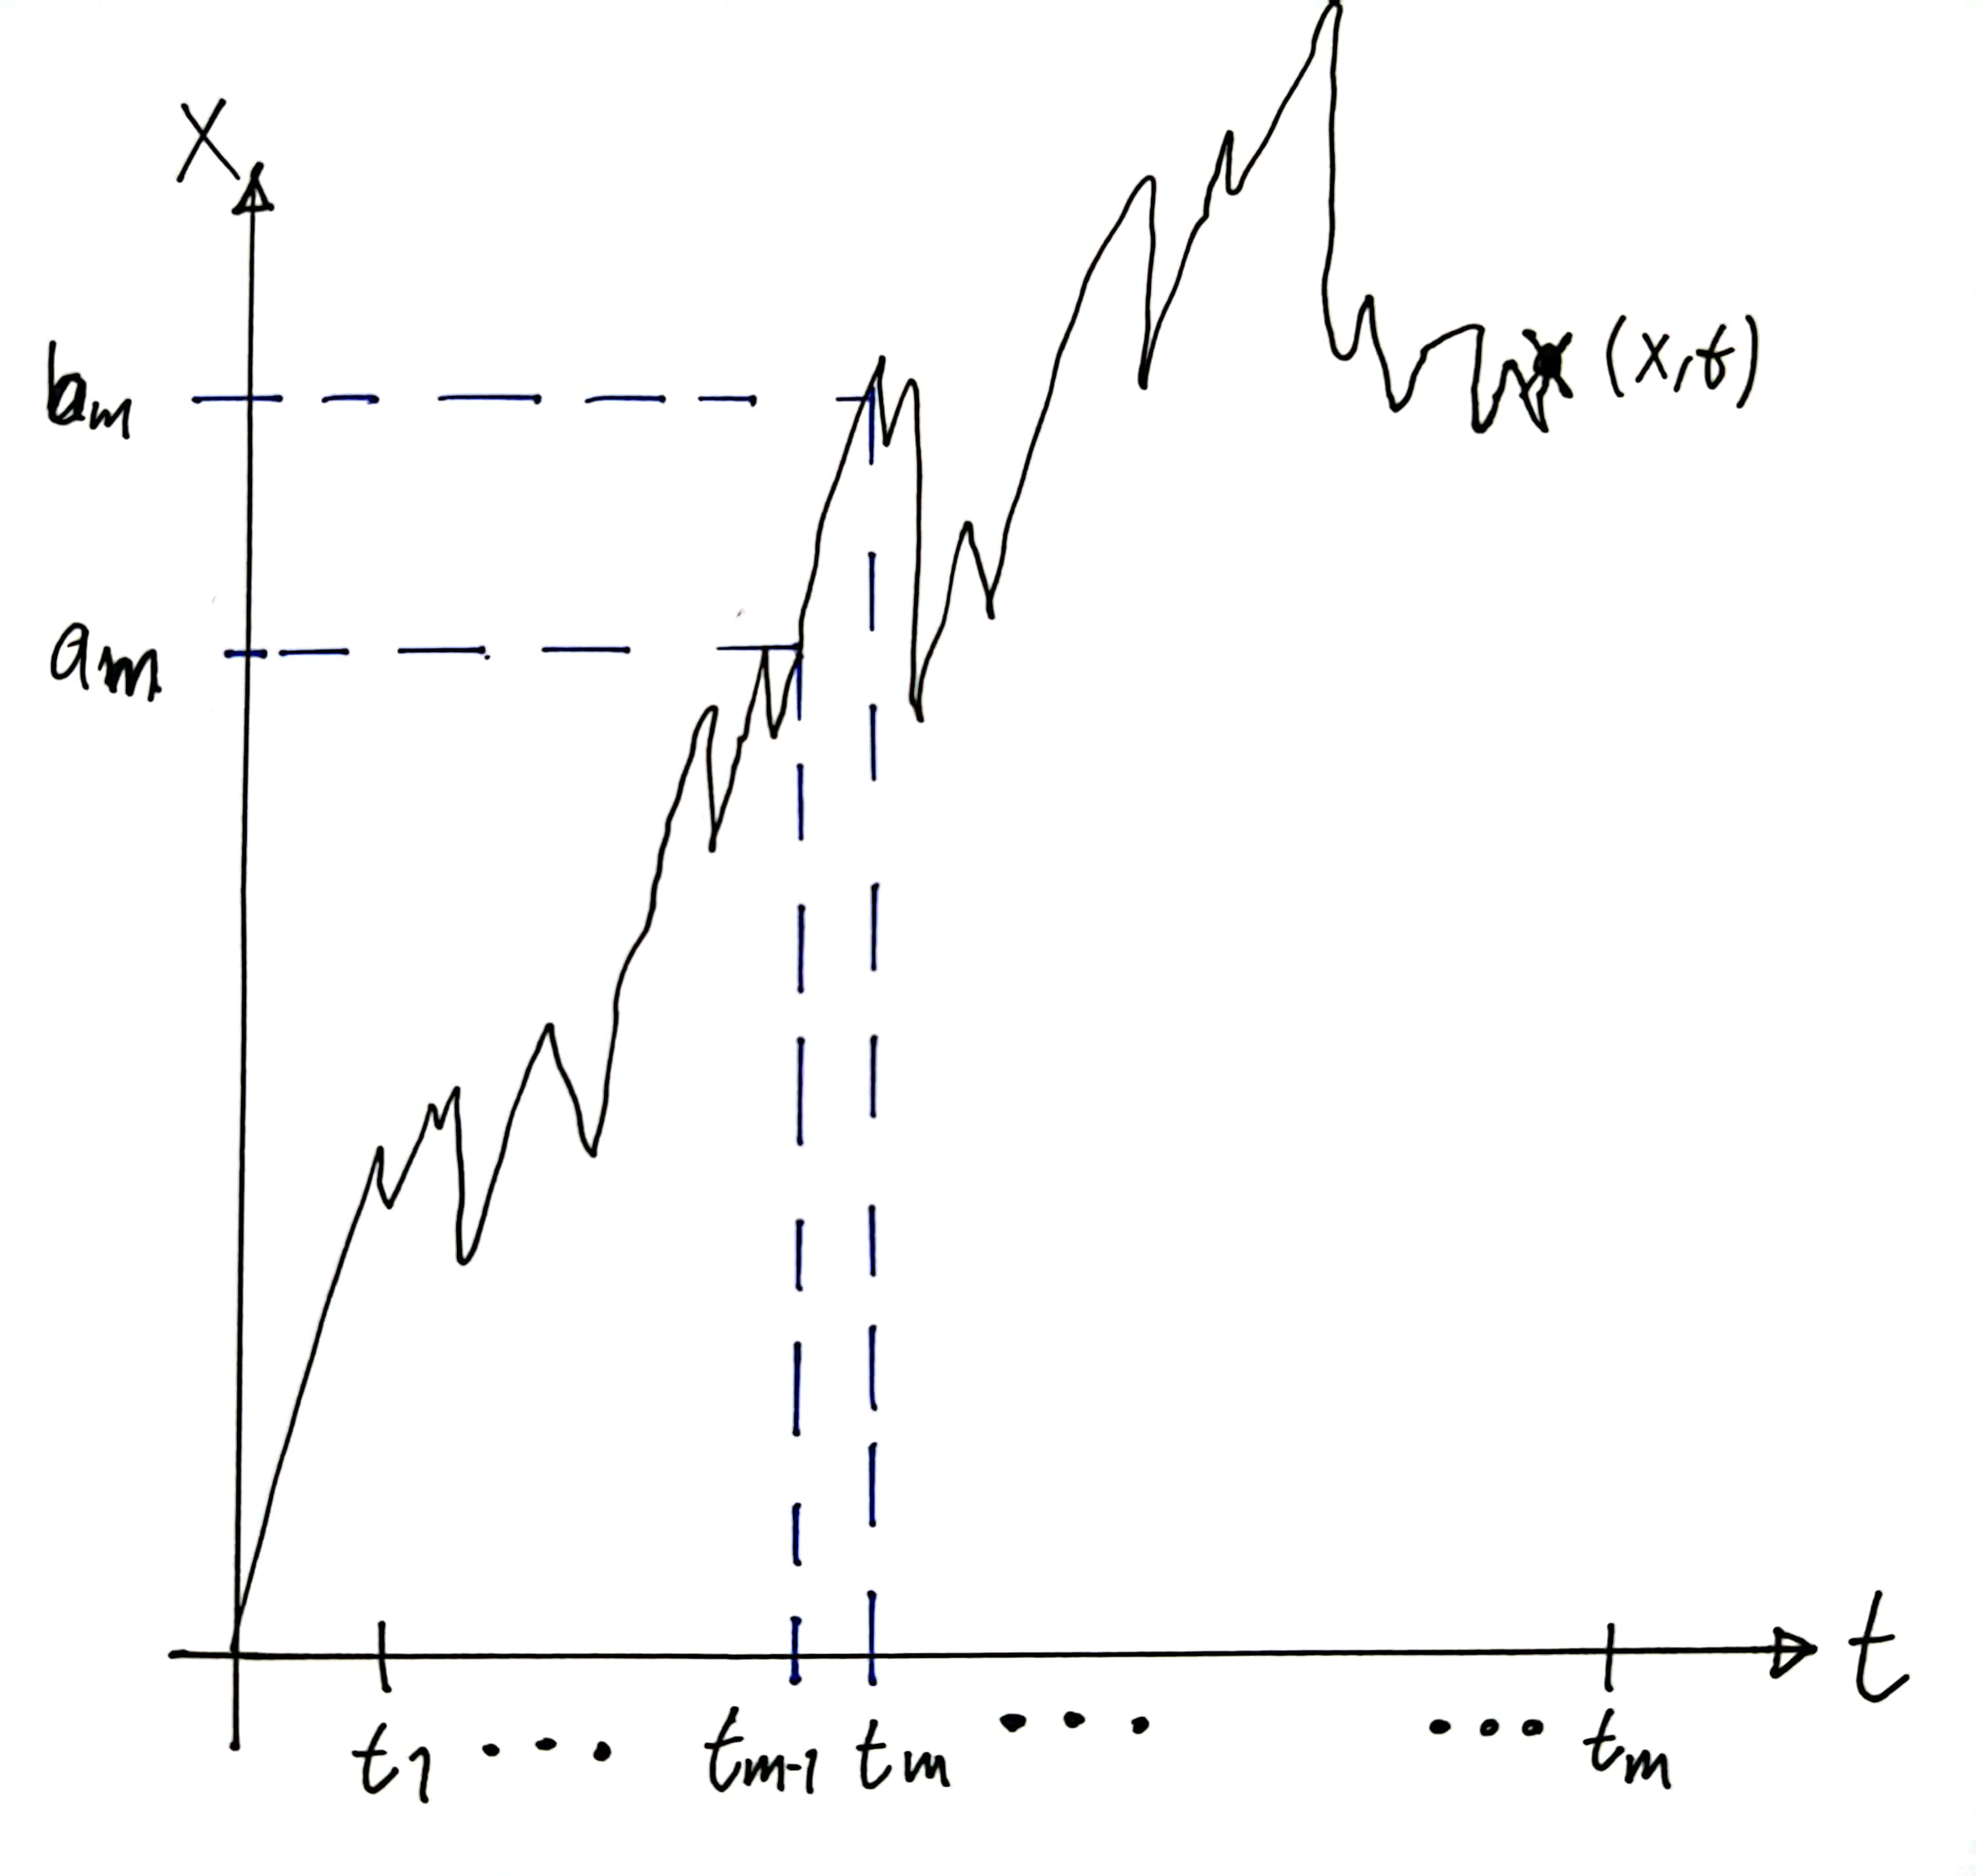
\includegraphics[width=.3\textwidth]{fig/path.jpg}
    \caption{A discretized path}
    \label{fig: path}
\end{figure}

As discussed around \autoref{eq: probability density}, when dealing with continuous space, and thus probability densities, the probability of finding a particle in the interval $(a, b)$ is
%
\begin{align}
    P(x\in (a, b), t ) = \int_a^b \dd x \, \Pe(\bm x, t).
\end{align}
%
To define probability density (``measure'') on an entier \emph{path}, and not just at isolated points, we discretize the path as
%
\begin{align}
    t_i &= i \Delta t, & i &\in [1, N], & t_N &= t, & x_i = x(t_i)
\end{align}
%
We consider paths with fixed endpoints, $x_0 = 0$, and $x_N = x$, as illustrated in \autoref{fig: path}.
A discretized path thus consists of finding the particle in certain intervals $(a_i, b_i)$ at times $t_i, i\in[1, N]$.
We define the probability measure of such a discretized path as
%
\begin{align}
    \Pe(x, t | x_i\in(a_i, b_i),\,  i \in 1, \cdots N )
    =
    \int\limits_{a_1}^{b_1} \dd x_1
    \cdots
    \int\limits_{a_{N-1}}^{b_{N-1}} \dd x_{N-1}\,
    \Pe(x, t | x_{N-1}, t_{N-1}) \cdots \Pe(x_{2}, t_{2} | x_{1}, t_{1}) \Pe(x_{1}, t_{1}) 
\end{align}
%
\todo[inline]{in the notes, the last integral is over $x_N$, but I assume it is $x_{N-1}$?}
Then, in the continuum limit, this becomes Brownian integral,
%
\begin{align}
    \D x(t)
    \equiv
    \lim_{\substack{|a_i-b_i|\rightarrow 0\\N \rightarrow \infty \\ t = \const}}
    \Pe(x, t | x_i\in(a_i, b_i),\,  i \in 1, \cdots N ).
\end{align}
%
This is a more careful definition of the path-integral measure defined in \autoref{section: introducing pi}.
In fact, this is a bone fide probability measure, as it has
%
\begin{enumerate}
    \item a \emph{sample space} (all paths)
    \item a $\sigma$-albebra \todo{define?}
    \item a measure on the sample space.
\end{enumerate}
%

\subsection*{Brownian functional}

Suppose $Q[x]$ is some \emph{functional} of the paths $x(t)$ with the form
%
\begin{align}
    Q[x] = \exp \left\{ - \int_0^t \dd \tau \, U(x(\tau)) \right\}.
\end{align}
%
We have already encountered such a functional in the Onsager-Machlup functional.
This is called a \emph{Brownian functional}.
In discretized form, this is a function $Q(x_1, \cdots x_{N-1})$.
Then, the expectation of this functional is\todo{Should we use $\E{\cdot } $ instead to be consistent?}
%
\begin{align}
    \mathbb{E}_{(x, t)}[Q]
    &
    \equiv
    \lim_{\substack{|a_i-b_i|\rightarrow 0\\N \rightarrow \infty \\ t = \const}}
    \int\limits_{a_1}^{b_1} \dd x_1
    \cdots
    \int\limits_{a_{N-1}}^{b_{N-1}} \dd x_{N-1}\,
    \Pe(x, t | x_{N-1}, t_{N-1}) \cdots \Pe(x_{2}, t_{2} | x_{1}, t_{1}) \Pe(x_{1}, t_{1}) 
    Q(x_1, \cdots x_{N-1}) \\
    &= \int\limits_{x(0) = 0}^{x(t) = x} \D x(t) \, Q[x].
\end{align}
%
We see immediately that $ \mathbb{E}_{(x, t)}[1] = 1$.


\chapter{Response field}
In this chapter, we will consider Langevin equations with the form
%
\begin{align}\label{eq: langevin for response}
    \odv{  }{ t } \phi(t)
    \overset{\alpha}{=}
    f(\phi(t)) + h(t) + \zeta(t),
\end{align}
%
where
%
\begin{align}
    \E{\zeta(t) \zeta(t')} = 2 T \delta(t - t').
\end{align}
%
This lecture is based on \footnote{\cite{hertzPathIntegralMethods2016}---\fullcite{hertzPathIntegralMethods2016}}, so we refer to these notes for the derivation---they are free to download.
This contains the calculations of correlation functions and response function,
%
\begin{align}
    C(t - t') &= \E{\phi(t)\phi(t')} \big|_{h=0}, &
    R(t - t') &= \fdv{ \E{\phi(t)} }{ h(t') } \bigg|_{h=0}
    =
    \frac{1}{2 T}
    \E{\phi(t)\zeta(t')} \big|_{h=0}.
\end{align}
%

As shown by \cite{hertzPathIntegralMethods2016}, the discretized version of \autoref{eq: langevin for response} is
%
\begin{align}
    \label{eq: discretized langevin for response}
    \phi_{n + 1} = \phi_n + \Delta t 
    \left\{
        (1 - \alpha) (f_n + h_n) + \alpha (f_{n+1} + h_{n+1})
    \right\} + \zeta_n
\end{align}
%
Here, $f_n = f(x(t_n))$ and $h_n = h(t_n)$, while
%
\begin{align}
    \zeta_n = \int_{t_n}^{t_{n+1}} \dd \tau \, \zeta(t).
\end{align}
%
With this, the \emph{generating functional} is
%
\begin{align}
    Z[\psi]
    \equiv
    \E{\exp \left\{ i \sum_n \psi_n \phi_n \right\}}
    =\int \dd \phi \, 
    \exp \left\{ - \Delta t \alpha \sum_{n=1}^M f'_n + i \sum_n \psi_n \phi_n  \right\}
    \times
    \frac{ 1 }{ \sqrt{ 4 \pi \Delta t T } }
    \exp \left\{ - \frac{ 1 }{ 4 T \Delta t } \sum_n \zeta_n^2(\phi) \right\}
\end{align}
%
where $\zeta_n(\phi)$ is given by \autoref{eq: discretized langevin for response}.
This is essentially the Onsager-Machlup functional~\autoref{eq:om_func}.

\note{%
    Add summary of renormalizing $R$.
}


\section{Supersymmetry}

We may extend the response field formalism by introducing \emph{Grassmann} variables $\xi_i$, which obey a certain symmetry: super-symmetry.
We briefly summarize the results here, the full details can be found in~\cite{hertzPathIntegralMethods2016}.

\subsection{Grassmann numbers}

We can define Grassmann numbers $\xi_i$ by the properties 
%
\begin{align}
    \xi_i \xi_j &= - \xi_j \xi_i, \\
    \xi_i (\xi_j \xi_k) &= ( \xi_j \xi_i) \xi_k,
\end{align}
%
\emph{anti-commuation} and \emph{associativity}.
As a consequence, $\xi^n = 0$, for $n > 1$.
Any function of a single Grassmann number therefore takes the form
%
\begin{align}
    f(\xi) = a + b \xi,
\end{align}
%
for constants $a$ and $b$, and in particular
%
\begin{align}
    e^\xi = 1 + \xi.
\end{align}
%
For functions of two variables,
%
\begin{align}
    f(\xi_1,\xi_2) = c_0 + c_1 \xi_1 + c_2 \xi_2 + c_{12} \xi_1 \xi_2,
\end{align}
%
and so on.


We may define the derivative by
%
\begin{align}
    \odv{  }{ \xi_i } \xi_j = \delta_{ij}.
\end{align}
%
This acts on the leftmost Grassmann number so
%
\begin{align}
    \odv{  }{ \xi_1 } f(\xi_1, \xi_1)
    &= c_1 + c_{12} \xi_2,&
    \odv{  }{ \xi_2 } f(\xi_1, \xi_1)
    &= c_2 - c_{12} \xi_1.
\end{align}
%
The derivative operators anti-commute.
Likewise, the integral is defined by
%
\begin{align}
    \int \dd \xi 1 &= 0,&
    \int \dd \xi \, \xi &= 1,
\end{align}
%
and
%
\begin{align}
    \int \dd \xi_1 \dd \xi_2 \xi_2 \xi_1
    = - \int \dd \xi_1 \dd \xi_2 \xi_1 \xi_2
    = 1.
\end{align}
%
With this, we may write the determinant of a matrix $A_{ij}$ as
%
\begin{align}
    \int \D \xi \D \bar \xi \exp \left\{ {\sum}_{ij} \bar \xi_i A_{ij} \xi_j \right\}
    = \det A,
\end{align}
%
where $\D\xi \D \bar \xi = \prod_{i} \dd \bar \xi_i \dd \xi$.
Furthermore,
%
\begin{align}
    \E{\xi_i \bar \xi_j}
    =
    \int \D \xi \D \bar \xi \exp \left\{ {\sum}_{ij} \bar \xi_i A_{ij} \xi_j \right\}
    = 
    A_{ij}^{-1}.
\end{align}
%

With this, we can write the determinant from integrating out the noise, $\zeta$, as integral over Grassmann numbers:
%
\begin{align}
    J[\phi]
    =
    \int \D \bar \xi \D \xi
    \,
    \exp \left\{ \sum_n
    \left[
        \bar\xi_n \left(1 - \alpha \Delta t f'_{n+1}\right)\xi_{n+1}
        - \bar\xi_n \left(1 - (\alpha - 1) \Delta t f'_{n}\right)\xi_{n}
    \right]
     \right\}.
\end{align}
%
This is then added to the action, and expectation values are now
%
\begin{align}
    \E{\bullet}
    = 
    \int \D\tilde \phi \D \phi \D \bar \xi \D \xi \, \bullet e^{-A},
\end{align}
%
where
%
\begin{align}
    &A = \\\nonumber
    &\sum_n
    \left\{
        T \Delta t \tilde \phi_n^2
        - i \tilde \phi_n \left(
            -\phi_{n+1} + \phi_n + \delta t\left[(1 - \alpha)f_n + f_{n+1}\right]
            \right)
            -
            \bar\xi_n \left[1 - \alpha \Delta t f'_{n+1}\right]\xi_{n+1}
            + \bar\xi_n \left[1 - (\alpha - 1) \Delta t f'_{n}\right]\xi_{n}
    \right\}.
\end{align}
%

\printbibliography

\end{fmffile}
\end{document}
